%__________________________________________________________________________________________ %
%-------------------------------------------PFC---------------------------------------------%
%__________________________________________________________________________________________ %


%%%%%%%%%%%%%%%%%%%%%%%%%%%%%%  PREAMBULO  %%%%%%%%%%%%%%%%%%%%%%%%%%%%%%%%%%%%%
% ----------------------Especificaciones de dise�o---------------------------- %

\NeedsTeXFormat{LaTeX2e}
\documentclass[12pt]{book}

\usepackage{a4}
\usepackage[Lenny]{fncychap}    % Estilos para capitulos
\usepackage{fancyhdr}           % Estilos para cabeceras
%\usepackage[spanish]{babel}
%usepackage[latin1]{inputenc}

% Para no tener problemas con las tildes
\usepackage[utf8]{inputenc}
\usepackage[english]{babel}

\usepackage{epsfig}
\usepackage{subfig}
\usepackage{epstopdf}
\usepackage{caption}
\usepackage{keyval}
\usepackage{graphicx}
\usepackage{float}              % Para poner las imags en cualquier sitio
\usepackage{listings}
\usepackage{color}
\usepackage{textcomp}
\usepackage{verbatim}
\usepackage{exceltex}



\definecolor{listinggray}{gray}{0.98}
\definecolor{lbcolor}{rgb}{0.98,0.98,0.98}
\lstset{
	backgroundcolor=\color{lbcolor},
	tabsize=3,
	rulecolor=,
	language=matlab,
	basicstyle=\footnotesize\sffamily,
	aboveskip={1.5\baselineskip},
	belowskip={1.5\baselineskip},
	columns=fixed,
	showstringspaces=false,
	extendedchars=true,
	breaklines=true,
	prebreak = \raisebox{5ex}[5ex][5ex]{\ensuremath{\hookleftarrow}},
	frame=none,
	showtabs=false,
	showspaces=false,
	showstringspaces=false,
	identifierstyle=\ttfamily,
	keywordstyle=\color[rgb]{0,0,1},
	commentstyle=\color[rgb]{0.133,0.545,0.133},
	stringstyle=\color[rgb]{0.627,0.126,0.941},
}

\usepackage[numbers,sort&compress,comma]{natbib}	% Modo de poner la bibliograf�a
\usepackage{verbatim}      %  \begin{comment}...\end{comment}
\usepackage{subeqnarray}   % equationarray with numbers 1a, 1b, ...
\usepackage{bbm}           % Para s�mbolo tipo n�meros reales. Ej: \bbm{R}
\usepackage{longtable}     % Para tablas largas de m�s de una p�gina
\usepackage{rotating}
\usepackage{psfrag}        % Para cambiar fragmentos de text en .eps por otro en latex
\usepackage{pifont}        % Para otros s�mbolos
\usepackage{fancybox}      % Para encuadrar texto en recuadros
\usepackage{amsmath}       % Mejora la calidad de las formulas
\usepackage{amsfonts}
\usepackage [linktocpage]{hyperref}      % Para enlaces de hipertexto
\usepackage{amssymb,amsfonts}
\usepackage{multirow}
\usepackage{booktabs}
\usepackage{color}
\usepackage{longtable}
\usepackage{float}
\usepackage{array}




\setcounter{tocdepth}{2}             % toc = table of contents. Para definir niveles del �ndice
\setcounter{secnumdepth}{5}          % Hasta cu�ndo se enumeran los caps, seccs, etc


\setlength{\topmargin}{-1.1cm}        % margen por arriba
\setlength{\parskip}{\baselineskip}
\setlength{\parskip}{0.3cm}          % Espacio entre parrafos
\setlength{\textwidth}{16.5cm}       % Ancho del �rea imprimible	
\setlength{\evensidemargin}{-0.4cm}  % Margen izdo en p�ginas pares
\setlength{\oddsidemargin}{0.3cm}    % Margen izdo en p�ginas impares
% evensidemargin = -oddsidemargin !!!

\setlength{\headsep}{1.0cm}
\setlength{\headheight}{3ex}
\setlength{\footnotesep}{5mm}
%\setlength{\mathindent}{1.0cm}       % Controla el espacio entre margen y ec si no est� centrada


%%% Definitionen f�r Fancy Headings
%\renewcommand{\baselinestretch}{3mm}
%\renewcommand{\labelenumi}{\roman{enumi}.}
%\renewcommand{\chaptermark}[1]{\markboth{#1}{}}
%\renewcommand{\sectionmark}[1]{\markright{\thesection\ #1}{}}
\renewcommand{\labelitemi}{$\bullet$}
\renewcommand{\labelitemii}{$\diamond$}
\renewcommand{\labelitemiii}{$\cdot$}

\lhead[\fancyplain{}{\thepage}]{\fancyplain{}{\sl\nouppercase\rightmark}}
\rhead[\fancyplain{}{\sl\nouppercase\leftmark}]{\fancyplain{}{\thepage}}
\cfoot{}
\pagestyle{fancyplain}  		% normale Kopfzeile; ohne Seitenzahl: empty

% Formato de capitulos
\ChTitleVar{\sf\Huge} % Tama�o de la letra del nombre del cap
\ChTitleAsIs


%%% Comando para quitar encabezado y pie de las pag en blanco
\newcommand{\clearemptydoublepage}
{\newpage{\pagestyle{empty}\cleardoublepage}}

\newcommand{\R}{\mathbb{R}}
\newcommand{\x}{\mathbf{x}}
\newcommand{\grad}{\hspace{-2mm}$\phantom{a}^{\circ}$} %para los grados centigrados

%%% Abstract
\newenvironment{abstract}
{\begin{center}
		\begin{minipage}{0.8\textwidth}
			\slshape}
		{\end{minipage}
	\end{center}}
	
	
	\typeout{ }
	\typeout{----------------------------------------------------------------------}
	\typeout{ }
	
	



%%%%%%%%%%%%%%%%%%%%%%%%%%%%%%  DOCUMENTO  %%%%%%%%%%%%%%%%%%%%%%%%%%%%%%%%%%%%%
%-------------------------Cuerpo del documento---------------------------------%


\begin{document}
	\renewcommand{\contentsname}{Contents}
	\renewcommand{\listfigurename}{List of figures}
	\renewcommand{\listtablename}{List of tables}
	\pagenumbering{roman}    % Numeraci�n de p�ginas con num romanos
	\setcounter{page}{1}      % Establece la siguiente p�gina como la 1
	\begin{titlepage}
\label{ch:cover}
\begin{center}

{\Large\textsc{Telecomunication Engeneering}}


Department:  \\ Signal Theory, Telematics and Communications

\textbf{University of Granada}


\vspace{0.5cm}

\begin{figure}[h]
	\centering
	
\epsfig{file=imagenes/ugr, width=7cm}
	\label{fig:ugr}
\end{figure}


\vspace{0.5cm}
\textbf{Master thesis}


\vspace{0.9cm}


{\Huge\textbf{Comparison of Posturographic Body-sway Measurements with Inertial Data of Parkinson Patients }}


\end{center}


\vspace{1.5cm}
\textbf{Written by:}  \hfill \textbf{Supervised by:}

Ver\'onica Torres S\'anchez \hfill    D. Juan Manuel Górriz Sáez(UGR)

							\hfill	  D. Javier Ramírez Pérez de Inestrosa (UGR)
							
							\hfill    D. Alberto Olivares Vicente (UMU)
							
							\hfill	  D. Kai Bötzel (UMU)


\end{titlepage}
		% Inclu�mos la portada en espa�ol
	\clearemptydoublepage
	
	%Declaración
%--------

\begin{titlepage}
\label{ch:Statement}
\vspace{2cm}

\noindent  D. Alberto Olivares Vicente, profesor  del dpto. de Teoría de la Señal, Telemática y Comunicaciones, como director del Proyecto Fin de Carrera de Dª. Verónica Torres Sánchez,

\vspace{2cm}
\noindent Informan:

\vspace{1.5cm}
\noindent Que el presente trabajo, titulado:

\noindent \textbf{Comparison of Posturographic Body-sway Measurements with Inertial Data of Parkinson Patients.}

\noindent Ha sido realizado y redactado por el mencionado alumno bajo nuestra dirección, y con esta fecha autorizamos a su presentación.
\vspace{3.5cm}

\noindent Granada, a 20 de julio de 2015 Fdo:

\vspace{6.5cm}
\noindent D. Alberto Olivares Vicente    \hfill   D. Juan Manuel Górriz Sáez

\end{titlepage}       % Incluimos la declaración del proyecto
	\clearemptydoublepage
	\begin{titlepage}
\label{ch:acknowledgements}
{ \huge \bfseries Acknowledgements \\[0.4cm] }


First and foremost, I would like to thank Dr Alberto Olivares Vicente and Juan Manuel Górriz Sáez for supervising this work, his assistance and most especially for his continuous motivation and encouragement.

Thanks to Robin Weiss for his suggestions, his great ideas and knowledge, his jokes when the work was being  hard and, in short, for helping me along this Project.

Special thanks go to my friends for valuing my work, encouraging me every day, their advices and making me smile with their crazy things. Of course, many thanks go to my friend and flatmate, for putting up with me in the work nights and making to laugh with their positive music .

Finally, I am deeply grateful to my family, for giving me the opportunity to study, respecting all my decisions and their motivation and affection.


\end{titlepage}       % Incluimos agradecimientos
	\clearemptydoublepage
	\begin{titlepage}
\label{ch:abstract}
{ \huge \bfseries Abstract \\[0.4cm] }

\end{titlepage}       % Incluimos resumen
	\clearemptydoublepage
	
\begin{titlepage}
\label{ch:abbrevations}
{ \huge \bfseries Abbrevations \\[0.4cm] }

\textbf{APA}: Anticipatory postural adjustments

\textbf{SIPBA}: Signal processing and Biomedical Applications

\textbf{FP}: force plate

\textbf{GW}: Gait Watch

\textbf{QS}: Qualysis System

\textbf{PD}: Parkinson’s disease

\textbf{IMU}: Inertial Measurement Unit

\textbf{MIMU}: Magnetic Inertial Measurement Unit

\textbf{EMG}: Electromyography

\textbf{MEMS}: Microelectromechanical Systems

\textbf{LTSD}: Long Term Spectral Detector

\textbf{FSD}: Framed Spectrum Detector

\textbf{COP}: center of pressure

\textbf{AP}: Antero-posterior

\textbf{ML}: Medio Lateral

\textbf{FIR}: Finite Impulse Response.


\end{titlepage}       % Incluimos abreviaciones
	\clearemptydoublepage
	
	\tableofcontents          % Pone índice
   \listoffigures		   	% Crea la lista de figuras
   \listoftables			% Crea la lista de tablas
	\clearemptydoublepage

	

	\clearemptydoublepage
	\chapter{Introduction}
\label{ch:Introduction}

\section{General}

\subsection{Parkinson's Disease}

According to Patients Medical \cite{patients_medical_definition_2014}, \begin{quote}``Parkinson's disease is a progressive, neurodegenerative disease that occurs when the neurons within the brain responsible for producing the chemical dopamine become impaired or die. Dopamine is essential for the smooth control and coordination of the movement of voluntary muscle groups. Once approximately 80\% of the brain's dopamine producing cells no longer function, the symptoms of Parkinson's disease begin to appear. [\dots] Parkinson's disease may be termed as a progressive movement disorder that is distinguished by marked slow movements, tremors, and unstable posture.''\end{quote}

Especially in advanced stages of the Parkinson's disease (PD)\nomenclature{PD}{Parkinson's disease} many patients exhibit an episodic, brief inability to step that delays gait initiation or interrupts ongoing gait. This phenomenon is called freezing of gait and is often associated with an alternating shaking of the knees, called knee trembling. However, these clinical signs of balance or gait problems are not evident in early stages of the disease \cite{mancini_anticipatory_2009}\cite{jacobs_knee_2009}.

\subsection{Anticipatory Postural Adjustments}

A major challange to the human ballance control system is the fact that we are bipeds having only one foot in contact with the ground while walking, and that two-thirds  of our body mass is located two-thirds of body height above the ground \cite{halliday_initiation_1998}. Thus, to induce stable gait anticipatory postural adjustments (APAs)\nomenclature{APAs}{Anticipatory Postural Adjustments} are necessary. The Encyclopedia of Neuroscience \cite[p.133]{woollacott_anticipatory_2009} defines APAs as "A predictive motor response that acts to counter, in a preemptive manner, the postural destabilization associated with a forthcoming movement." As seen in Figure \ref{fig:APAoverview} the centre of body mass (COM)\nomenclature{COM}{Centre of Mass} is accelerated forward and laterally over the stance foot to make sure that the body does not fall laterally toward the stepping foot during the swing phase \cite{woollacott_anticipatory_2009}.  The curve of the centre of pressure (COP)\nomenclature{COP}{Centre of Pressure} is divided in three periods. Period S1 indicates the uncoupling of the COP and COM as the COP moves posteriorly and toward the intended stepping limb. Then, in the S2 period, the COP displaces mediolaterally toward the stance foot. Finally, during the S3 period the COP moves anteriorly under the stance foot \cite{hass_gait_2005-1}.

\begin{figure}
	\centering
	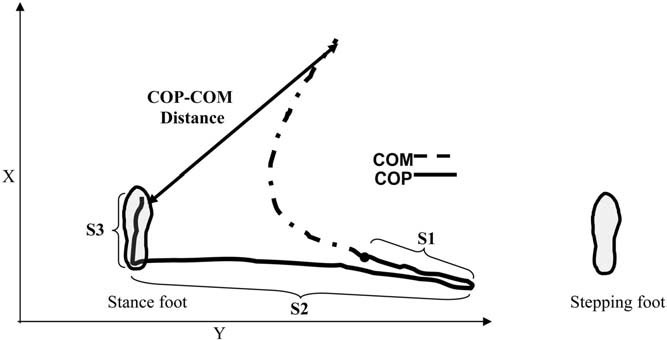
\epsfig{file=images/APA_overview, width=9cm}
	\caption{Anticipatory Postural Adjustments during forward-oriented gait initiation when stepping with the right foot \cite{hass_gait_2005-1}.}
	\label{fig:APAoverview}
\end{figure}


\section{Goals}

The goal of the project was to analyse anticipatory postural adjustments prior to step inition and subsequently build a classifier using MATLAB, which is fed with data from both a force plate and a magnetic inertial measurement unit (GaitWatch \cite{olivares_vicente_gaitwatch_2013}) to distinguish between Parkinson patients and healthy subjects. To gather the data the subject stood in front of the force plate. Then the GaitWatch and force plate record was started and the subject made a step onto the force plate. After standing a variable time of two to ten seconds the subject left the force plate, made a few steps, turned left und stopped in front of it again. This sequence was repeated ten times.


\section{Motivation}

Advanced PD can increasingly diminish quality of life, since patients are dependent on help from others to accomplish daily tasks. New drugs are currently being developed and are expected to decelerate or stop the course of the disease in early stages \cite{botzel_motivation_2014}. Thus, a quantitative PD classification enabling early diagnosis of the disease could optimise early treatment and could help to validate new treatment methods. Additionally, an objective evaluation of longterm treatment success was ensured.


\section{State of the art}

There are several methods and devices to assess Parkinson's disease and to analyse anticipatory postural adjustments. They differ in terms of practicability, accuracy, validity, portability, and cost. The state of the art at the beginning of the project is described below.

\subsection{Rating scales}

A commonly used rating scale is the Unified Parkinson’s Disease Rating Scale (UPDRS),\nomenclature{UPDRS}{Unified Parkinson’s Disease Rating Scale} which is a short test performed by a physician \cite{klerk_long-term_2009}. The patient is rated on 31 different items (see Table \ref{tab:UPDRS}) with a score of 0 (normal) to 4 (severely affected). Another method is the rough, but widely utilised and accepted Hoehn and Yahr scale (HY)\nomenclature{HY}{Hoehn and Yahr scale}. Parkinsonian motor impairment is categorised in 5 stages: Unilateral (Stage 1) to bilateral disease (Stage 2) without balance difficulties, to the presence of postural instability (Stage 3), loss of physical independence (Stage 4), up to being wheelchair- or bed-bound (Stage 5) \cite{goetz_movement_2004}. Without the need of complex technical devices these tests are relatively simple to perform. \citeauthor{klerk_long-term_2009} \cite{klerk_long-term_2009} mentioned their disadvantages, including subjectivity, short observation periods, and unfamiliarity of the environment that both rating methods bring along.

\begin{table}[h]
\begin{tabular}{lll}
\hline
Mentation, mood & Activities of daily & Motor examination \\
and behavior & living & \\
\hline
Intellectual impairment & Speech & Speech \\

Thought disorder & Salivation & Facial expression\\

Depression & Swallowing & Tremor at rest \\

Motivation/initiative & Handwriting & Action or postural tremor of hands \\

& Use of eating utensils & Rigidity \\

& Dressing & Finger taps\\

& Hygiene & Hand movements\\

& Turning in bed & Rapid alternating movements of hands\\

& Falling & Food agility\\

& Freezing when walking & Arising from chair \\

& Walking & Posture\\

& Tremor & Gait\\

& Sensory Complaints & Posture stability\\

& & Body bradikinesia and hypokinesia \\
\hline
\end{tabular}
\caption{Unified Parkinson's Disease Rating Scale items adapted from \cite{herndon_handbook_2006}.}
\label{tab:UPDRS}
\end{table}

\subsection{Instrumentation}

In addition to the aforementioned subjective rating scales, there are different devices used to quantify gait and posture and assess them objectively. All of them come with certain pros and cons. The following devices have been used:

\subsubsection{Electromyographs} Electromyography is a technique for evaluating the electrical activity of skeletal muscles. Successive action potentials generated by muscle cells are measured, by means of needle electrodes inserted into the muscles, and displayed on a cathode-ray oscilloscope. Thus medical abnormalities can be detected. The instrument used to capture the visual recording, termed electromyogram, is called electromyograph \cite{encyclopedia_britannica_electromyography_2014}. Electromyography is constrained to clinical application only, but gives indication about the contribution of specific, individual muscles to APAs.

\subsubsection{Force plates} Force plates quantify the ground reaction force (GRF)\nomenclature{GRF}{Ground Reaction Force}, which is the force exerted to the human body by the ground. The GRF is a three-dimensional vector with three orthogonal components. One component along the direction of gravity, one parallel to the ground in the sagittal plane, and one parallel to the ground in the frontal plane. Those are vertical planes that divide the body in left and right halves, and ventral and dorsal sections, respectively. A force plate usually gives an electrical voltage proportional to the force in each of the three directions. Force plates can be characterised according to the following criteria: Sensitivity in Volts per Newton, crosstalk (indication of vertical force if a horizontal force is applied and vice versa), repeatability (similar results under the same load), and time- and temperature drift \cite{griffiths_principles_2006}. Froce plates are limited to clinical application, too. They have the advantage that they don't have to be calibrated.

\subsubsection{Inertial measurement units} Devices that use a combination of inertial sensors like accelerometers and gyroscopes are referred to as inertial measurement units (IMUs)\nomenclature{IMU}{Inertial Measurement Unit}. If they also include magnetic field sensors (magnetometers), they are called magnetic inertial measurement units (MIMUs)\nomenclature{MIMU}{Magnetic Inertial Measurement Unit}. With these devices the orientation of the body can be obtained with up to nine degrees of freedom, provided that triaxial accelerometers and magnetometers are used, respectively \cite{olivares_vicente_signal_2013}.

\begin{itemize}

\item \textsc{Accelerometers} measure the acceleration of an object relative to an inertial frame. Since acceleration cannot be measured directly, the force exerted to a reference mass is obtained and the resultant acceleration is computed according to Newton's second law $ \mathbf{F} = m \cdot \mathbf a $ \cite{encyclopedia_britannica_accelerometer_2014}.

\item \textsc{Gyroscopes} measure angular velocity and are based on the Coriolis Effect. By means of integration of the angular velocity the rotation angle is obtained \cite{olivares_vicente_signal_2013}.

\item \textsc{Magnetometers} measure the strength and the direction of the magnetic field in a point in space, using the relationship between magnetic fields, movement and induced currents \cite{olivares_vicente_signal_2013}.
 
\end{itemize}
MIMUs are portable and relatively inexpensive. They can be easily attached to the body and thus allow non-clinical longterm application. Their drawbacks are complex calibration procedures and drift behaviour over time, depending on intensity and duration of the movement. Hence, in order to maintain a satisfactory degree of precision, periodical recomputation of the calibration parameters is required \cite{olivares_vicente_signal_2013}.

\subsection{Classification}

There are several research works in the literature dealing with APA analysis and PD classification, as the evaluation of posture and gait are key components of the clinical evaluation of PD \cite{palmerini_classification_2013}.

\citeauthor{klerk_long-term_2009} \cite{klerk_long-term_2009} developed a measurement system called PD Monitor, implementing an Activity Classifier that quantifies tremor and bradykinesia in the arm, thigh, and trunk, in an ambulant way and over long periods of time. They validated their measurements with video records, which were rated by physicians using the UPDRS and concluded that ``the PD monitor can be used for a detailed evaluation of the PD motor symptoms in order to optimize treatment.'' \cite{klerk_long-term_2009}.

\citeauthor{mancini_anticipatory_2009} \cite{mancini_anticipatory_2009} found that the 11 untreated early-to-middle stage Parkinson's patients that took part in their study have a significantly smaller peak COP displacement towards the stepping leg and peak trunk acceleration towards the stance leg compared to the 12 age-matched healthy control subjects. Even though step velocity and step length were not different. The results show that lateral APAs are impaired in early, untreated PD and that they are detectable with inertial sensors. As well as force plate-based, also acceleration-based extracted features can be used to detect impairments equally well. Due to the fact that the acceleration signal can be easily obtained via a sensor on a belt, no matter if in clinical or home environment, APA detection by means of accelerometers is considered as a useful way to characterise patients in early stage of PD without evident clinical symptoms. Additionally in \cite{mancini_anticipatory_2009} it is proposed to carry out further studies to determine the relationship between small APAs and the probability to develop start hesitation and freezing.

\citeauthor{palmerini_classification_2013} \cite{palmerini_classification_2013} states that PD classfication could deliver a tool to follow the progression of the disease during the entire course to examine the efficiency of treatment. They studied classification of PD subjects  using triaxial accelerometers on the lower back at L5 level and an ad hoc wrapper feature selection technique and achieved satisfactory accuracy of 93.75\%. Twenty early-mild PD subjects and 20 healthy age-matched control subjects had to perform two simple tests (quiet standing, Timed Up and Go test), in two evaluations over a 1-year follow-up, to test accuracy and robustness over time. As well as \cite{mancini_anticipatory_2009} they found that lateral dynamics i.e. range of motion are impaired in early-mild PD and suggested further investigation on validity of measures in later stages.

\section{Document structure}


	\clearemptydoublepage
	\chapter{Hardware Description}
\label{ch:Hardware}
Along this chapter we will introduce a general description of all devices used to data gathering for the development of this project.


It should be noted at this point that there are two clearly differentiated parts. In the first of them, we work with Force Plate and GaitWatch data, taking out their characteristic signals and synchronising them. In the second of them, we work jointly with Gait Watch and Qualisys System data for the purpose of comparing the accuracy in the calculated orientation angles.


\section{GaitWatch}

GaitWatch is an Inertial Measurement Unit (IMU) designed for gait monitoring of patients. It was developed by Prof. Dr. Med. Kai B¨otzel at the Department of Neurology of Ludwig-Maximilians University in Munich in conjunction with Dr. Alberto Olivares Vicente from the Department of Signal Theory, Telematics and Communications of the University of Granada. \cite{OlivaresBotzel2013}

The system is composed of the central processing unit and
a set of measuring units which are wired to it. The measuring units are 
placed in the patients’ thighs, shanks, arms and trunk.

The central processing unit has a microcontroller is in charge of gathering the data from the external measurement units and writing it to the memory card. So, this central unit is placed in the trunk inside a box and it contains an AL-XAVRB board with an AVRATxmega processor which contains the necessary embedded firmware to gather the data from all the measurement units and store it in a microSD card. Also, the trunk box contains some embedded magnetic and inertial sensors.

There are three different kinds of external units with the following components:
\begin{itemize}
	\item Type A (thighs and shanks): 
	\begin{itemize}
		\item IMU 5 from Sparkfun. IMU 5 contains an IDG500  biaxial gyroscope (from which only Y axis is actually used) with a measurement range of $\pm500deg/s$ and a $\pm3g$ triaxial accelerometer, ADXL335 .
	\end{itemize}
	\item Type B (arms):
	\begin{itemize}
		\item IDG500  biaxial $\pm500deg/s$ gyroscope.
	\end{itemize}
	\item Type C (trunk box):
	\begin{itemize}
		\item ADXL345  triaxial accelerometer with programmable range ($\pm16g/\pm8g/\pm4g/\pm2g$).
		\item IMU3000 triaxial gyroscope with programmable range ($\pm250/\pm500/\pm1000/\pm3000 (deg/s)$).
		\item Micromag3  triaxial magnetometer ($\pm11Gauss$).
	\end{itemize}
\end{itemize}


\section{Force Platform}

\section{Qualisys System}
	\clearemptydoublepage
	\chapter{Gait Watch and Force Plate signals processing}
\label{ch:GWandFP}

\section{Introduction and chapter's structure}
Along this chapter we will introduce the protocol used to obtain the Gait Watch and Force Plate signals as well as the developed software to synchronise and analyse the signals that characterise the anticipatory postural adjustments before gait.

On the one hand, we carry out the synchronisation between the signal from inertial sensors (Gait Watch) and the force signals from the platform. It's very important for comparing both devices, determining the differences and similarities and finally resolving if we can obtain the same information from both systems.

On the other hand, we’ll analyse the most interesting signals to characterise the APAs, obtaining the parameters of them which may be of interest.


\section{Data gathering Protocol}
Prior to start of data gathering, it’s necessary to set up the protocol for procedure that patients have to carry out while the data are recorded. The establishing this procedure is very important so that the synchronisation works properly because we have to identify a clear movement in both signals to match one signal with the other at the same time.
In addition, the realised movements must be representatives to obtain conclusive data which help us to extract characteristics for the purpose of identify differences between patients and control subjects subsequently.

The steps followed by the patients are detailed hereafter:

1.	Subject stands in front of the Force Plate.

2.	Gait watch record starts for data gathering.

3.	Force plate record starts for data gathering.

4.	Subject makes a step onto the platform.

5.	Subject stands on the platform a variable time between 2 and 10 seconds.

6.	Subject makes some step  forward and turns left to stand in front of the platform again.

This procedure is repeated ten times by each subject in order to characterise better the movement made.
It’s important to clarify that the GaitWatch recording contains all these ten episodes ( in other cases more) and the platform recording only contains one episode each. So, this is a fact that we have to consider to do the synchronisation.

\section{Synchronisation}

\subsection{Introduction and chapter's structure}
One of the most important aspects whether you have data acquired from multiples devices or channels is the synchronisation. If these data are not appropriately correlated or synchronised, the analysis and conclusions from your use will be erroneous. Also, it’s very important doing all automatically when you have a data on a broad scale.
Therefore, the following sections explain how the information has been obtained and processed automatically, as well as what features have been calculated to characterise the movements of the patients and to carry out the synchronisation between the Force Plate signals and GaitWatch signals. This content is superficially depicted in \ref{fig:diagramSynchronisation}.

\begin{figure}[H]
	\centering
	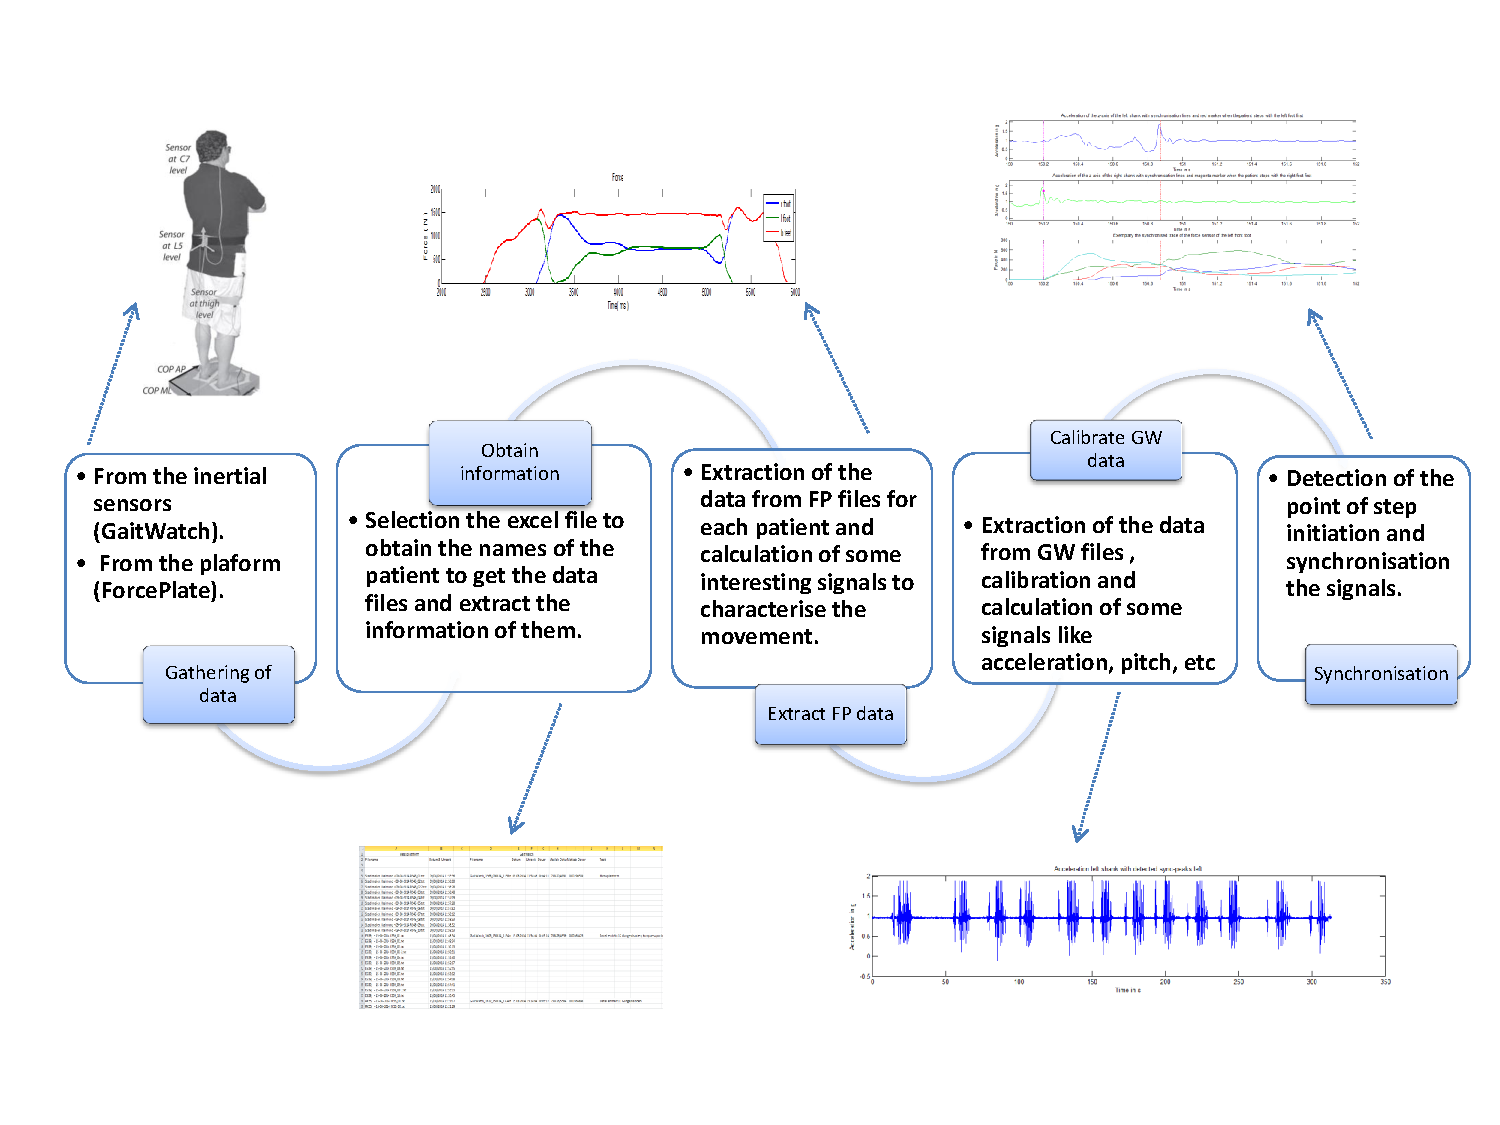
\epsfig{file=imagenes/diagramSynchronisation.pdf, width=15cm}
	\caption{Diagram of the Synchronisation's progress.}
	\label{fig:diagramSynchronisation}
\end{figure}

\subsection{Design of developed code  in Matlab}
\subsubsection{Selection, reading and obtaining of information from the excel file}
All patients data , that is, the different files have been generated after the gathering (  of the force plate as well as Gait Watch), gathering date, duration of the experiment and other observations are saved in a Excel file. 

In order to automate all as much as possible, the code is in charge of extraction of the necessary data (files names) to carry out the appropriate calculations for each patient. This is done once the Excel file has been selected, thus, it have to have a specific structure to be able to read the data correctly.

At the end of this fraction of code, we save all file names of both systems (force plate and Gait Watch) corresponding to each patient, in order to access and extract them posteriorly.

\subsubsection{Extraction of the forceplate data}
As we said before, the  force plate data files are recorded independently each others, that is, there is a *.txt file for each repeat.
Each file contains the force data of the toes and heels of both feet. It really realises a distribution of the sensors to cover these four segments\ref{fig:Force4signals}. Every measure is obtained for each point of time according to the sample frequency. Also, this file contains the force data from each cell that is part of platform in each frame\ref{fig:pseudocolor}.

\begin{figure}[H]
	\centering
	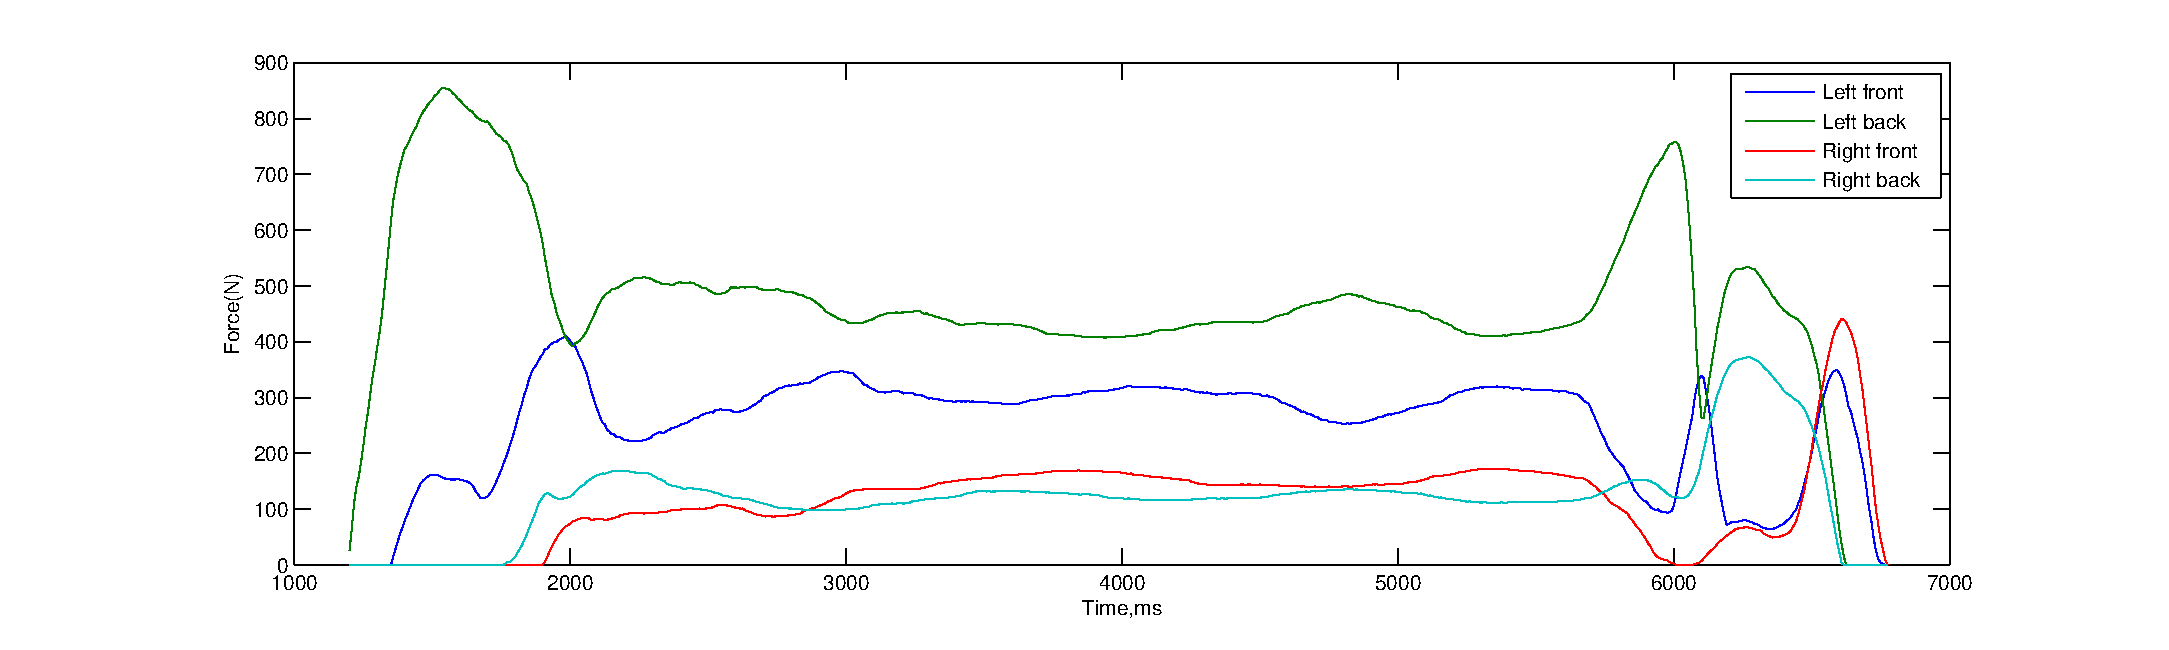
\epsfig{file=figures/Synchronisation/Force4signals, width=18cm}
	\caption{Force in each body segment.}
	\label{fig:Force4signals}
\end{figure}

\begin{figure}[H]
	\centering
	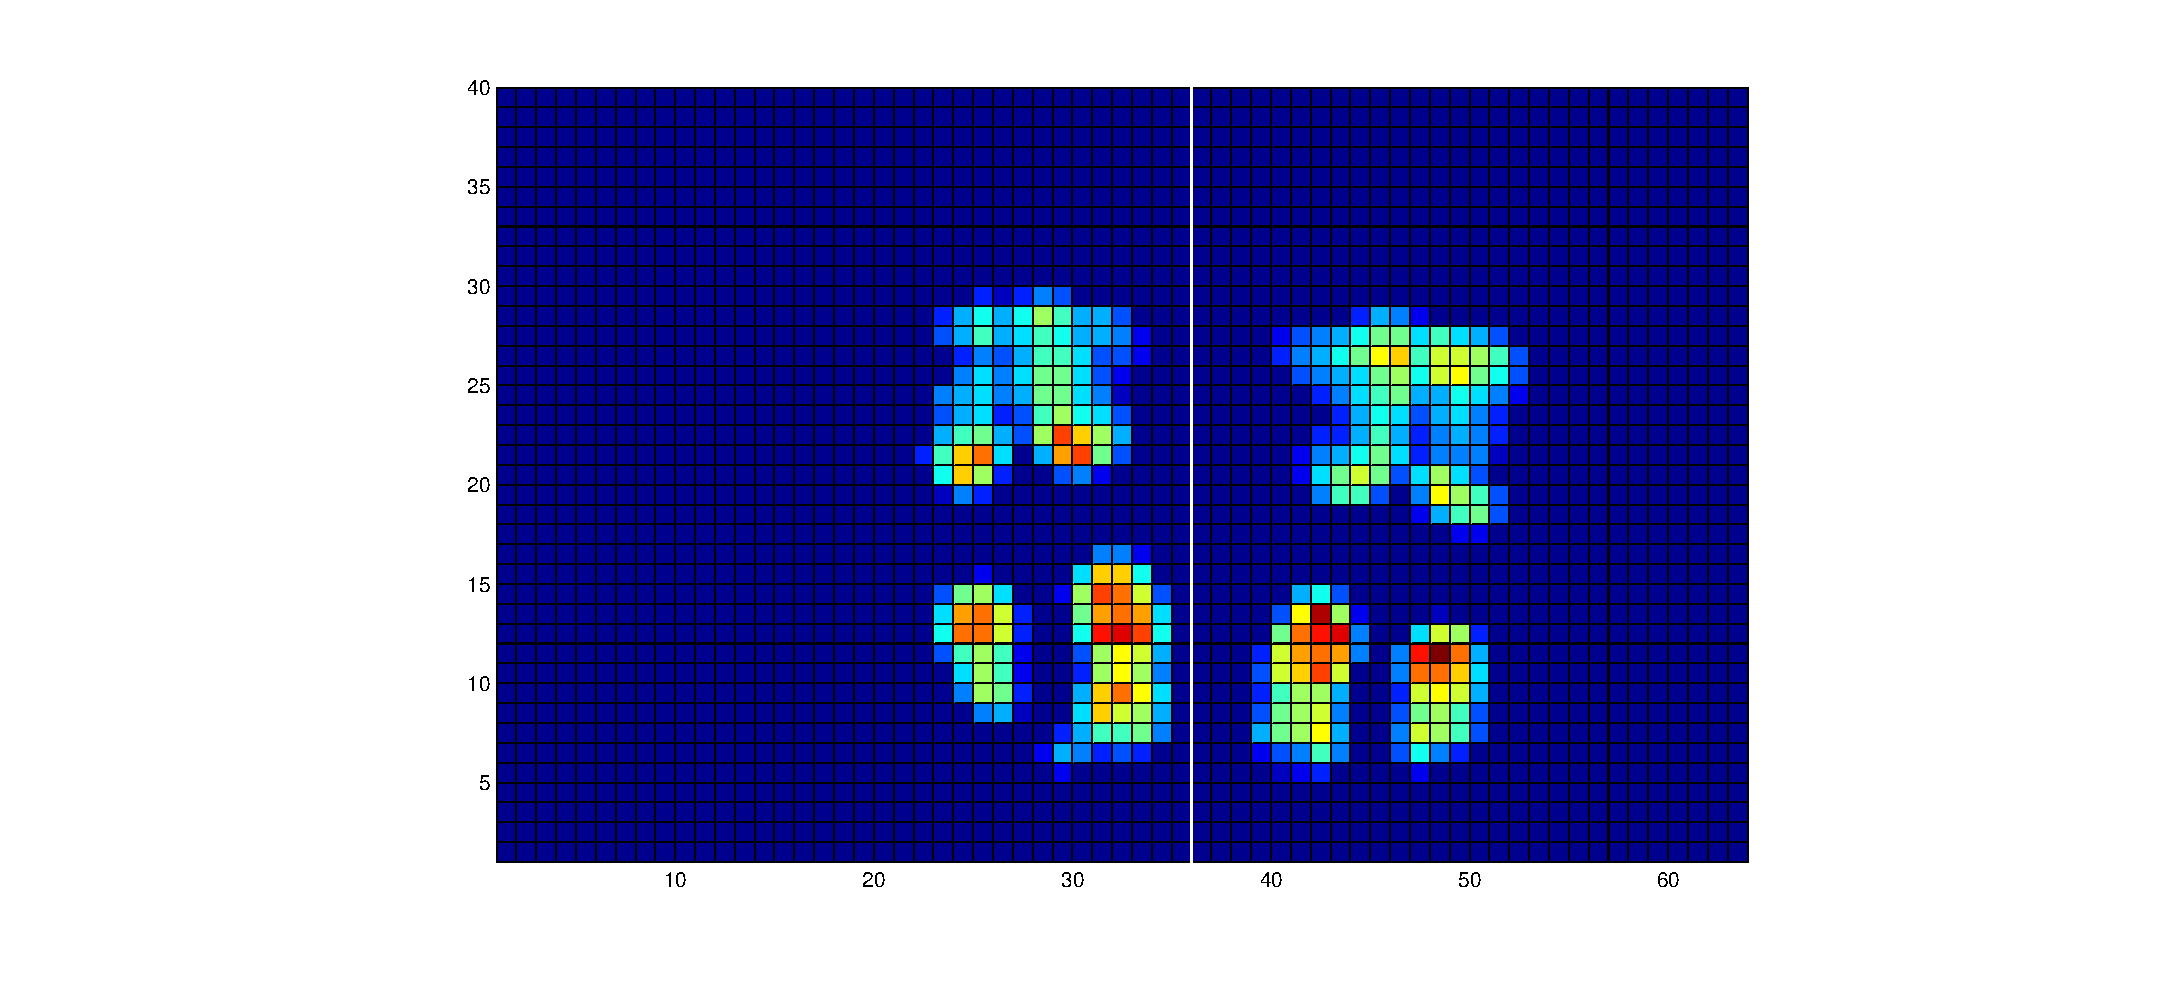
\epsfig{file=figures/Synchronisation/pseudocolor, width=18cm}
	\caption{Pseudocolor with the force in each cell of the platform}
	\label{fig:pseudocolor}
\end{figure}

Once we recover this data, some parameters are calculated for the movement characterization carried out over the platform. 

\begin{itemize}
	\item \textbf{Midline}: it represents the midline between both feet. This is important to find the gap between feet and it gives us a idea of their position in the platform. Thus, we carry out the sum of cells force in the anterior-posterior direction. So, this line is in the minimum between two maximum corresponding to the position of both feet. We use this parameter to calculate the center of pressure.
	\begin{figure}[H]
		\centering
		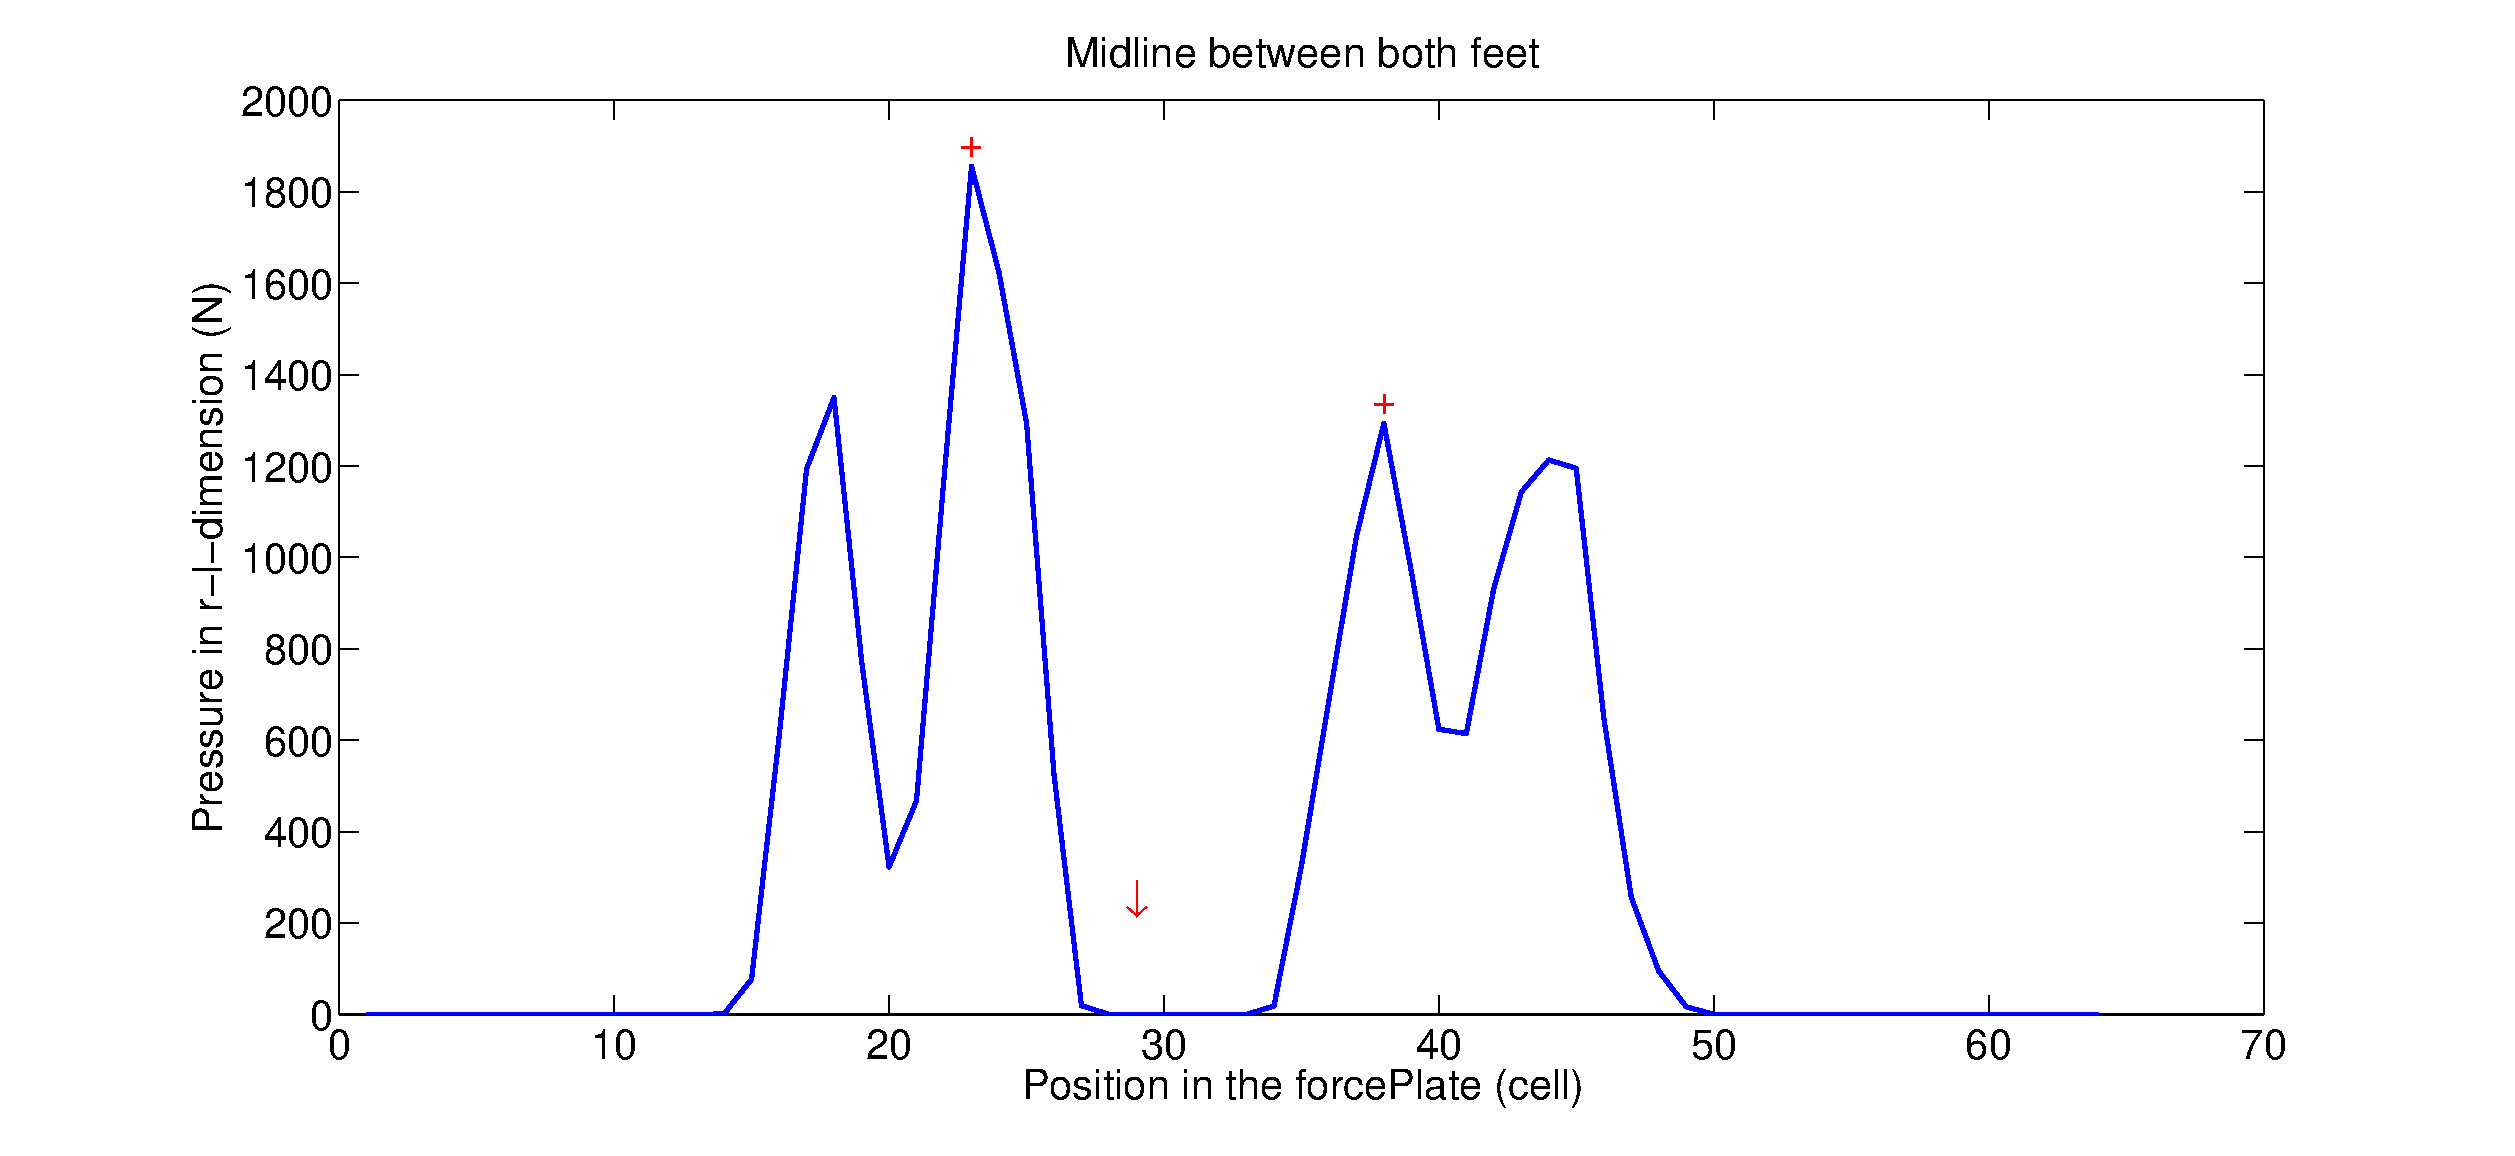
\epsfig{file=figures/Synchronisation/midlineForceplate, width=18cm}
		\caption{Midline between both feet in platform.}
		\label{fig:midlineForceplate}
	\end{figure}
	
	\item \textbf{The total force in the platform for each point of time}: This signal is useful to do the synchronisation due to we can determine clearer when the patient touches the plate.
		\begin{figure}[H]
			\centering
			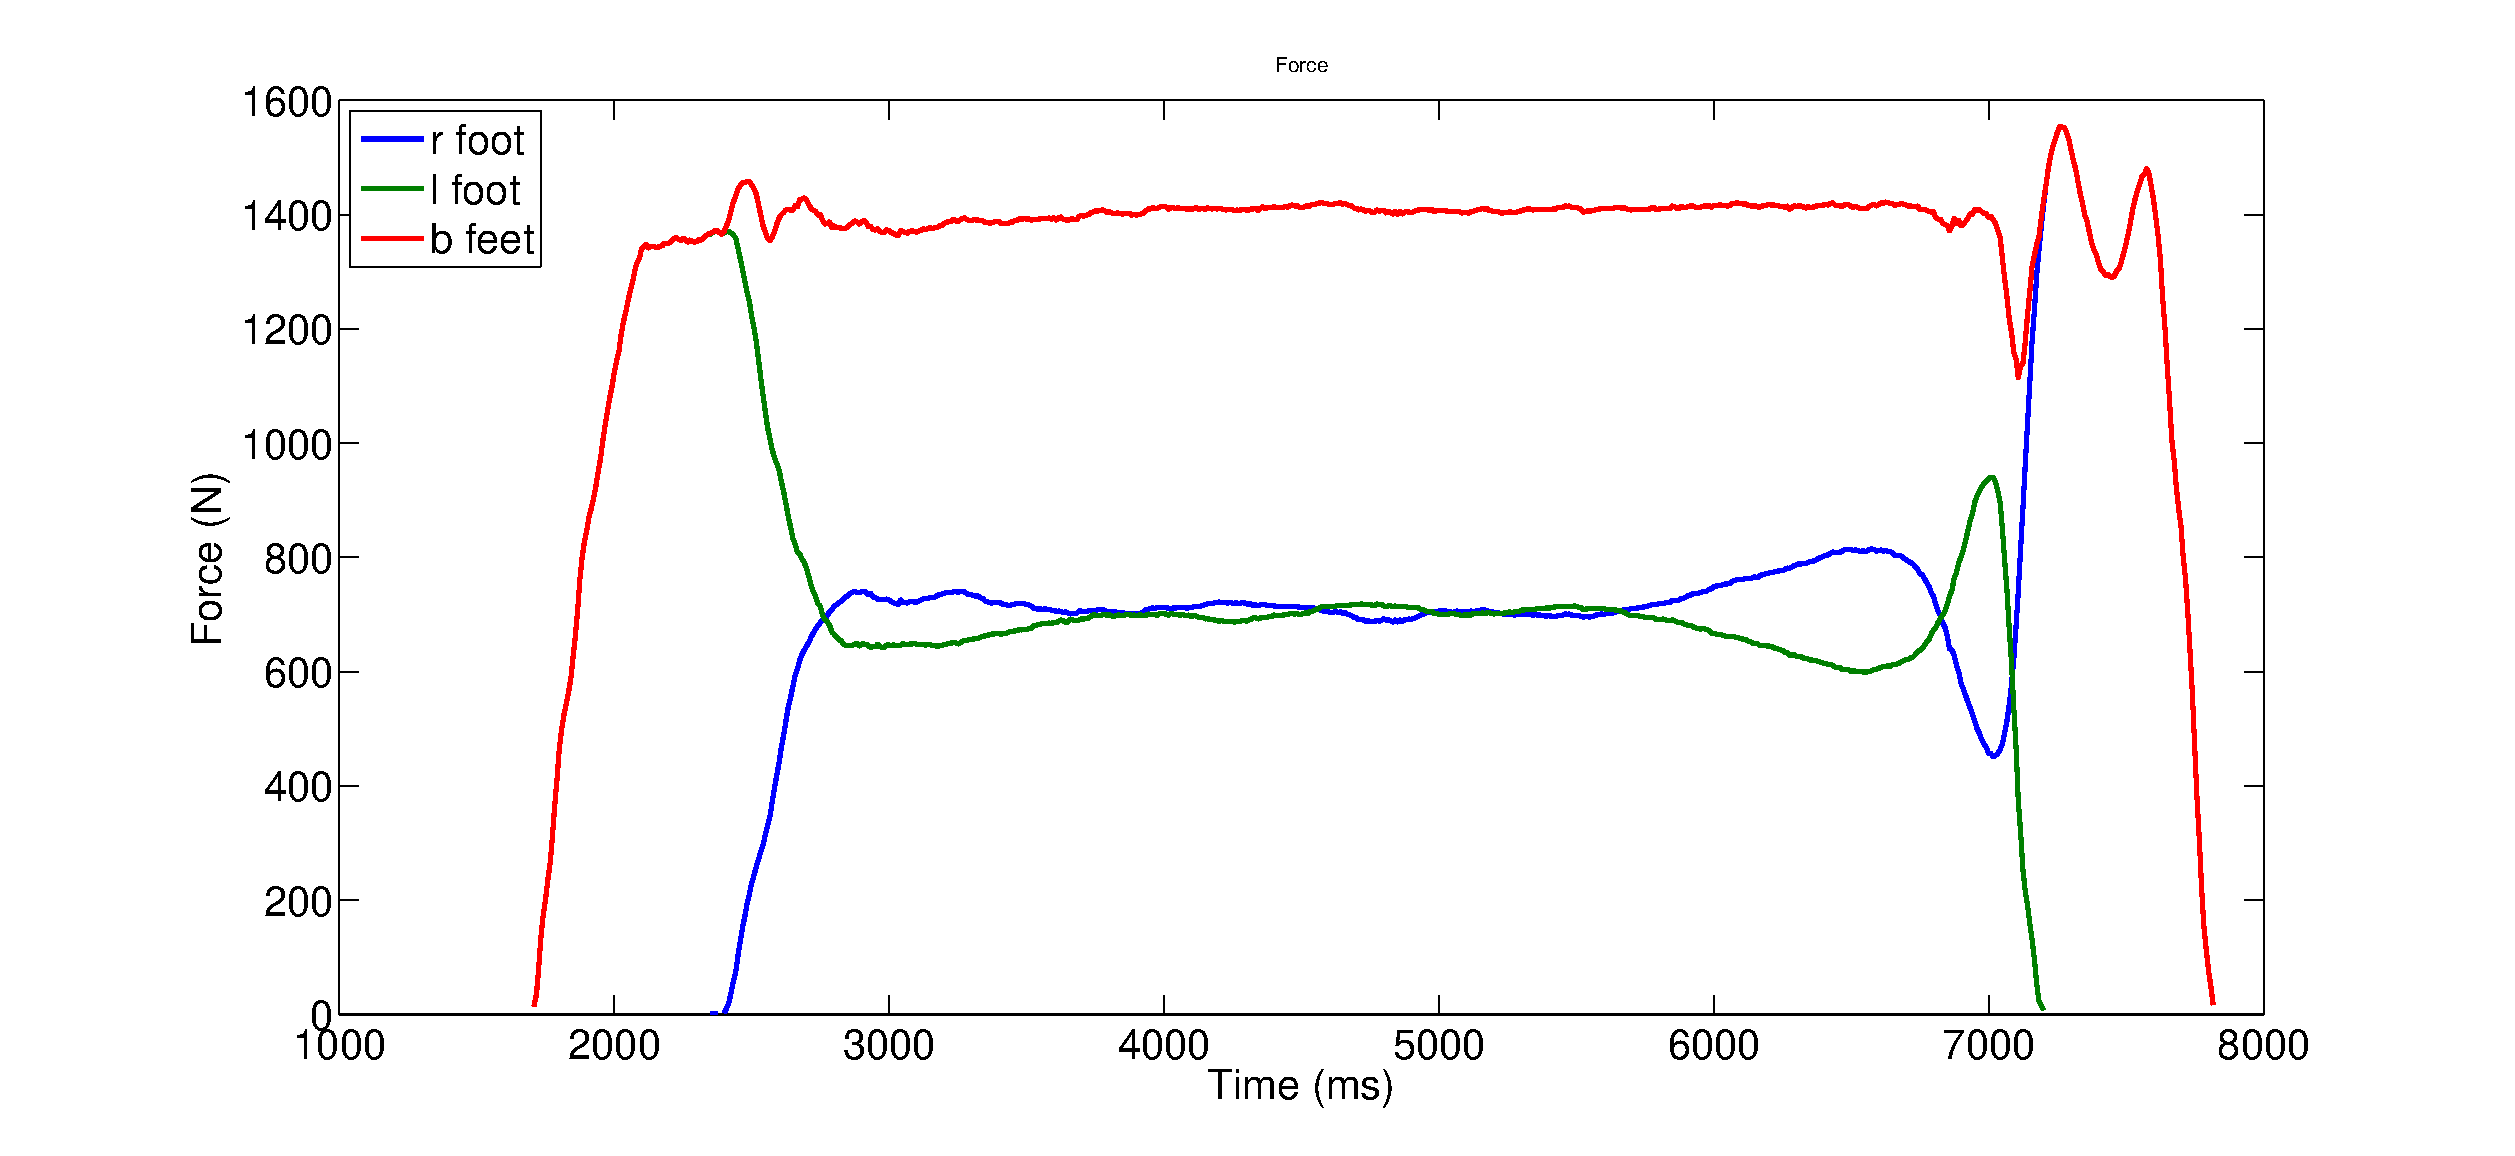
\epsfig{file=figures/Synchronisation/forceFP, width=18cm}
			\caption{Total force in the platform of the right, left and both feet.}
			\label{fig:forceFP}
		\end{figure}
	
	\item \textbf{Antero-posterior COP}: center of pressure in forward-backward direction.
		\begin{figure}[H]
			\centering
			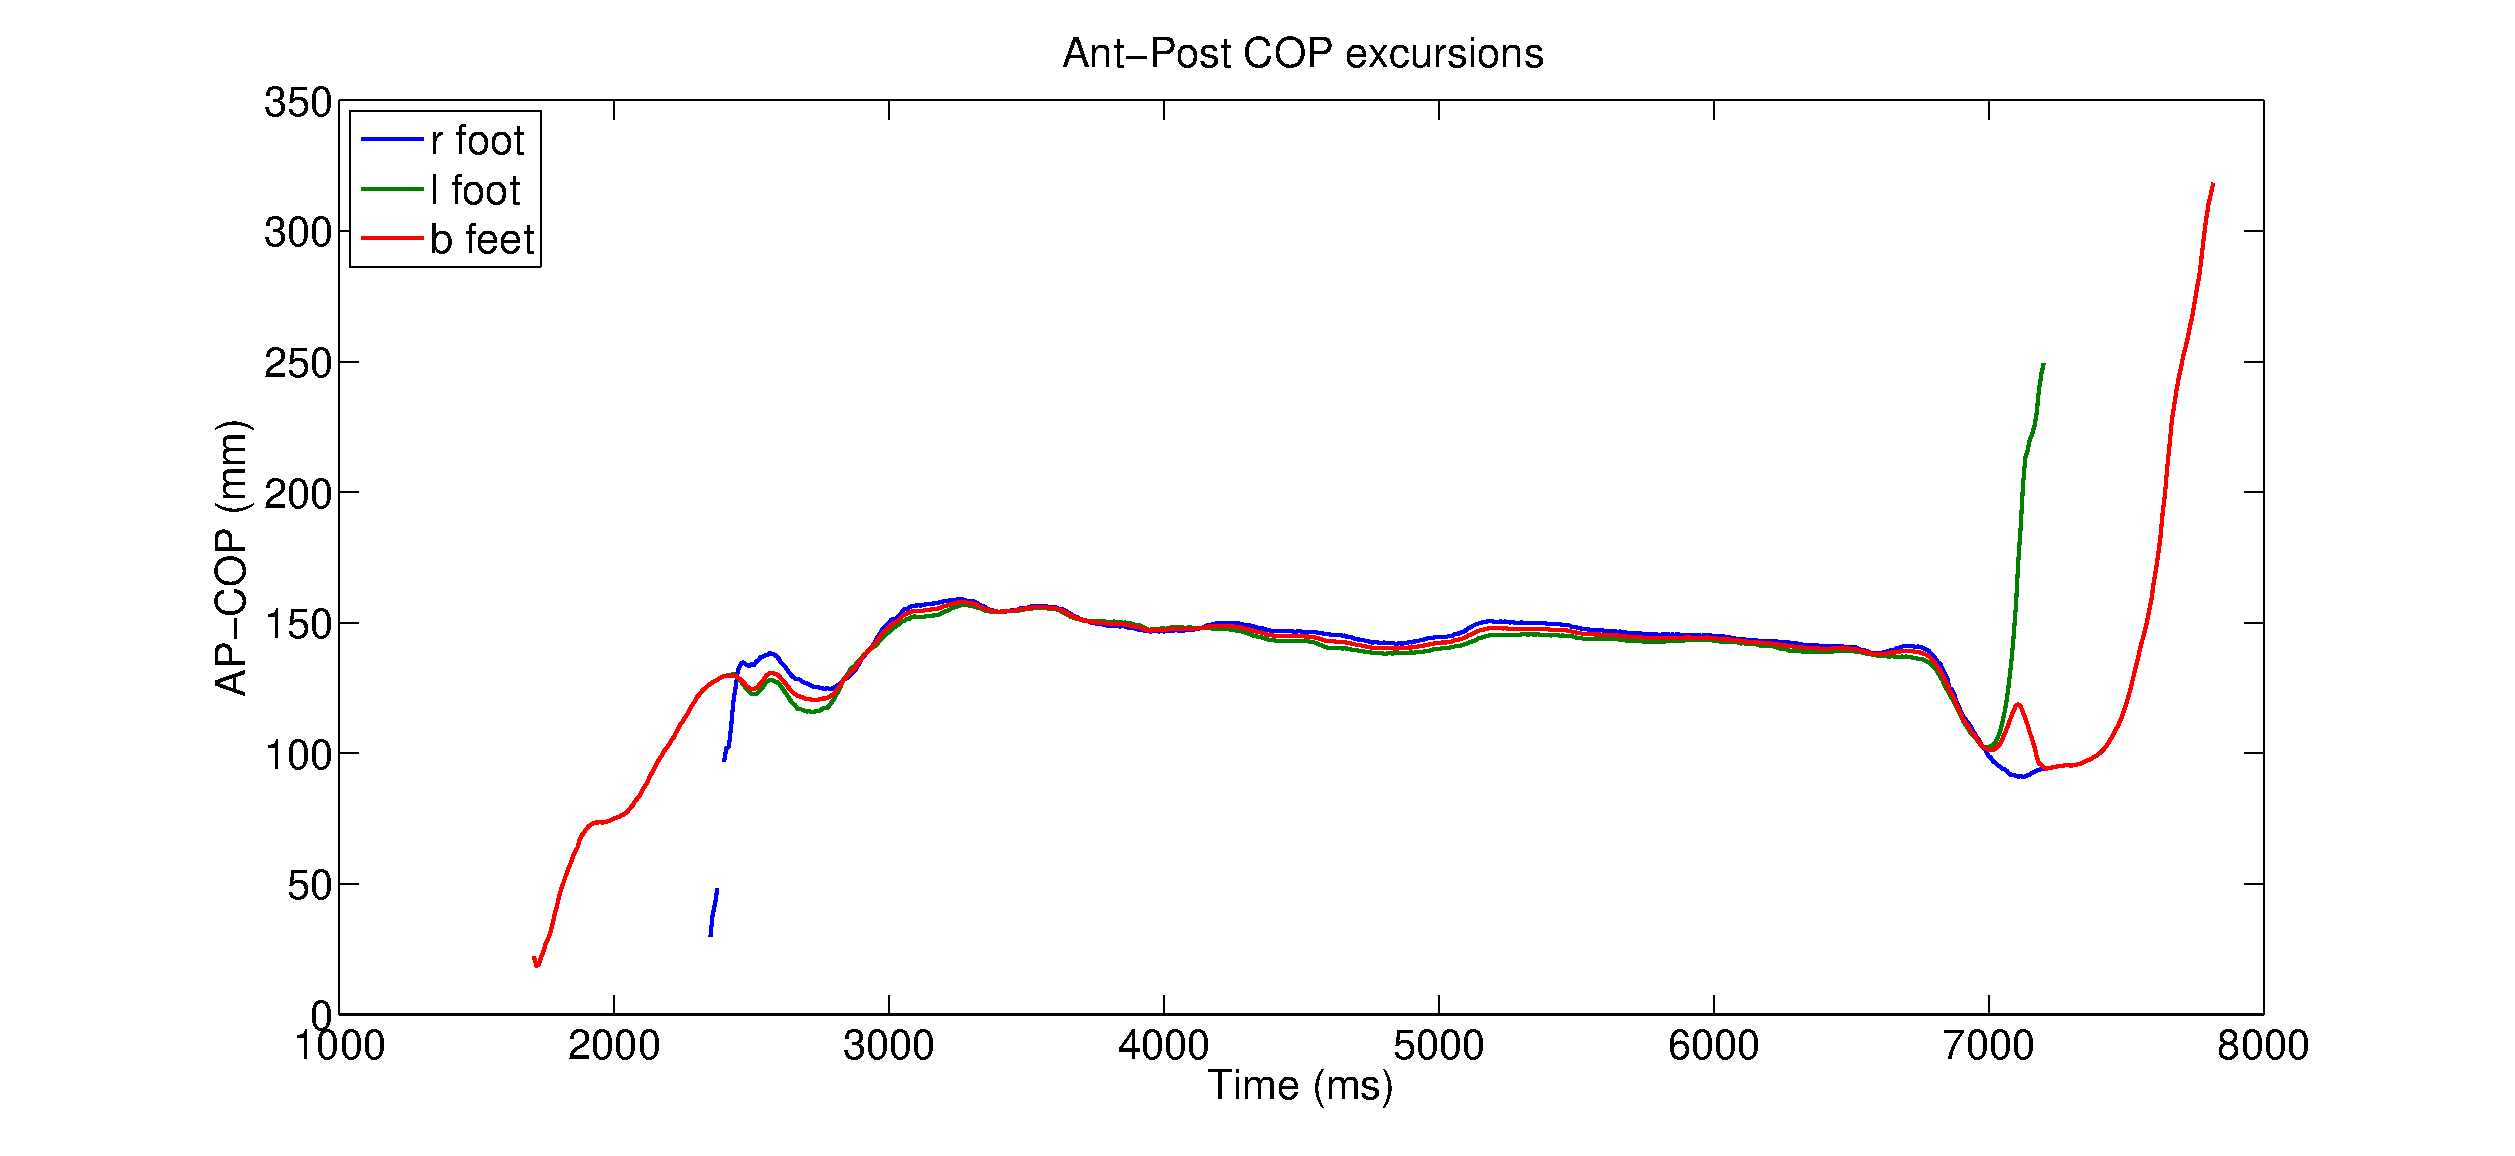
\epsfig{file=figures/Synchronisation/APCOP, width=18cm}
			\caption{Center of Pressure in Antero-Posterior direction.}
			\label{fig:APCOP}
		\end{figure}	
	
	\item \textbf{Medio-lateral  COP}: center of pressure  in right and left direction.
			\begin{figure}[H]
				\centering
				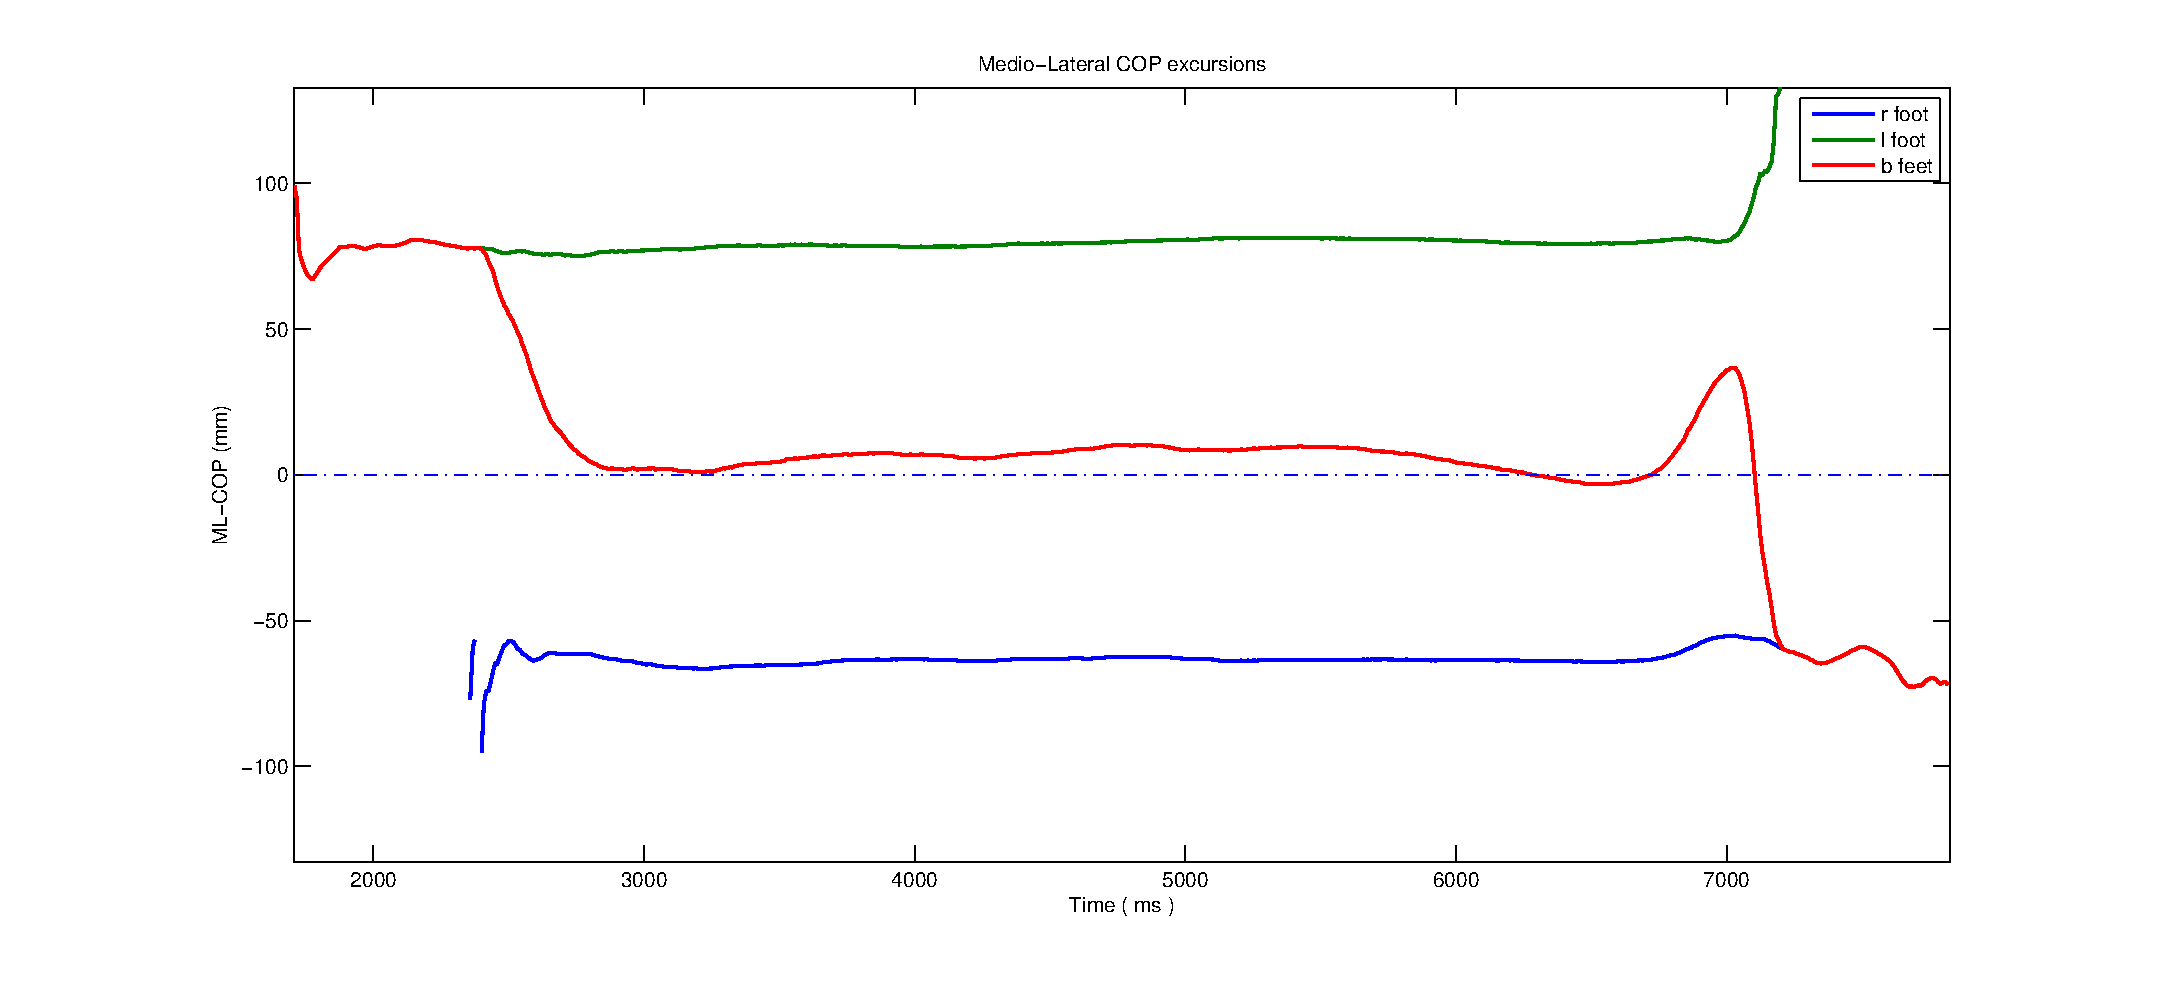
\epsfig{file=figures/Synchronisation/MLCOP, width=18cm}
				\caption{Center of Pressure in Medio-Lateral direction.}
				\label{fig:MLCOP}
			\end{figure}
	
\end{itemize}

Center of pressure can be expressed as follows:

\begin{equation}
	\label{COP}
	R=\sum_{i}^{n}m_{i}r_{i}
\end{equation}


Where R is the “Center of pressure”, M is the total force and mi are the force that are located in space with coordinated ri, in this case, in the plane. This location (ri) is calculate with respect to the midline.

These signals help us to characterise Anticipatory Postural Adjustments  before gait.  APAs indicate the movement or swinging of body before walk or carry out some movement. Thus, these are the interesting  measures to compare between each repeat as well as each patients to characterise the movement, determine if there is a pattern and figure out the differences and similarities between them.

All these signals are saved for each cycle in a single variable corresponding to the patient.


\subsubsection{Calibration of the GaitWatch data}
When we are working with sensors, calibration is one of the most important aspect that needs to be carried out. Prior to the calibration process,
the information at the sensors  will be a signal composed of integer
numbers  or real numbers bounded into a range which is determined by the precision of the sensors and converters. These numeric values lack of physical value, so it is absolutely necessary to convert them into a scale that can be measured in physical units.

The sensors present several errors due to some effects like scale factor may not be linear or the triad isn’t perfectly orthogonal. To remove these undesired effects, the software include a model to compensate this before the calibration. 
To do so, we have used the code made by Dr. Alberto Olivares Vicente in his doctoral thesis\cite{A.Olivares2013}, with minor modifications of his work.

Besides the unwanted effects mentioned above, the output of magnetometers is distorted by wide band measurement noise appearing several large peaks of noise in the signals. To remove this automatically, we used a threshold considering that these peaks are much greater than the mean of the signal \ref{fig:GWErrorDetected}.

\begin{figure}[H]
	\centering
	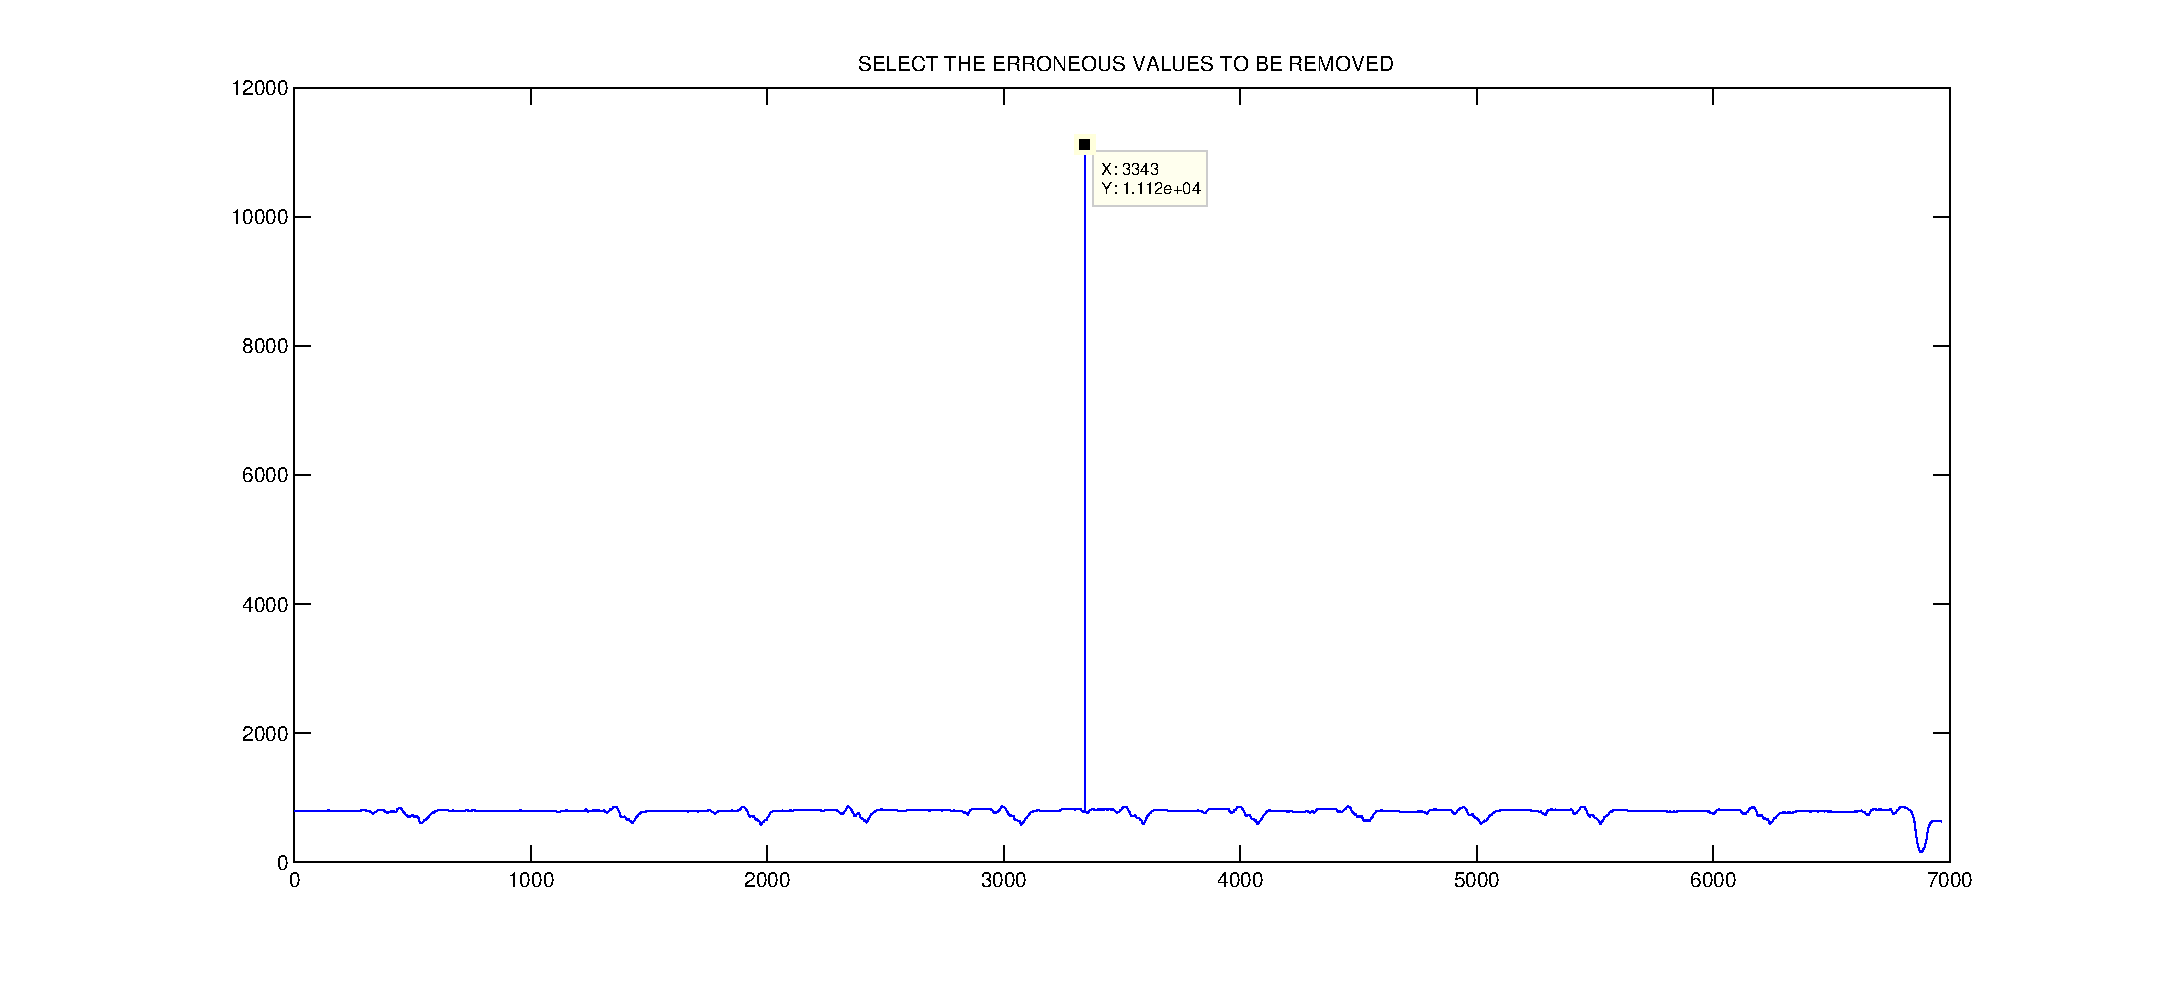
\epsfig{file=figures/Synchronisation/GWDetectErrorValueAutomatically, width=18cm}
	\caption{Value erroneous in magnetometer signal detected automatically.}
	\label{fig:GWErrorDetected}
	\end{figure}

The erroneus values in the magnetometer signal are removed sustituting these samples by the subsequent value unless the erroneous value is in the last position of the singal, in which case it is substituted by the preceding value.

\subsubsection{Synchronisation}	
In this section we will explain how we carried through the synchronisation of the Force Plate and GaitWatch signals and the considerations adopted to do it properly.

The first step is to detect when the step happens in both systems. In order to do this, we’ll use the completed force from Force Plate system and shank acceleration from the Gait Watch accelerometer. We chose these signals because it’s easy to see in them the point when the patients step.

Once we have selected the right signals to do the synchronisation we have to differentiate each cycles in the acceleration signal because we have all repeats together in the same file. To do this, we used activity detection code implemented by Dr. Alberto Olivares Vicente in his Doctoral thesis. Figure \ref{fig:activityDetection} shows the result.

In addition we did a comparative study testing two different methods based on the  computation of the spectrum (Fourier Transform) of the input signal. Also, we tried several input signal to determine which is the best option to do the motion detection in this case.

We will use the Long Term Spectral Detector (LTSD) \cite{Ramirez2004} and a variation of this called Framed Spectrum Detector (FSD). Spectrum-based methods have been used in others kinds of applications like Voice Activity detection \cite{Ramirez2006}\cite{Ramirez2007} and activity sequences detection such as running or sitting-standing up\cite{A.Olivares2013} .

The technical difference between LTSD and FSD is that the first of them compute the Long term spectral Envelope whereas FSD uses the spectrum of each frame  in which the input signal is divided\cite{A.Olivares2013}. What we observe when we use them in our signals is that the results are better when we use LTSD instead of FSD method  in the most of the cases\ref{fig:activityDetection}.

\begin{figure}[H]
	\centering
	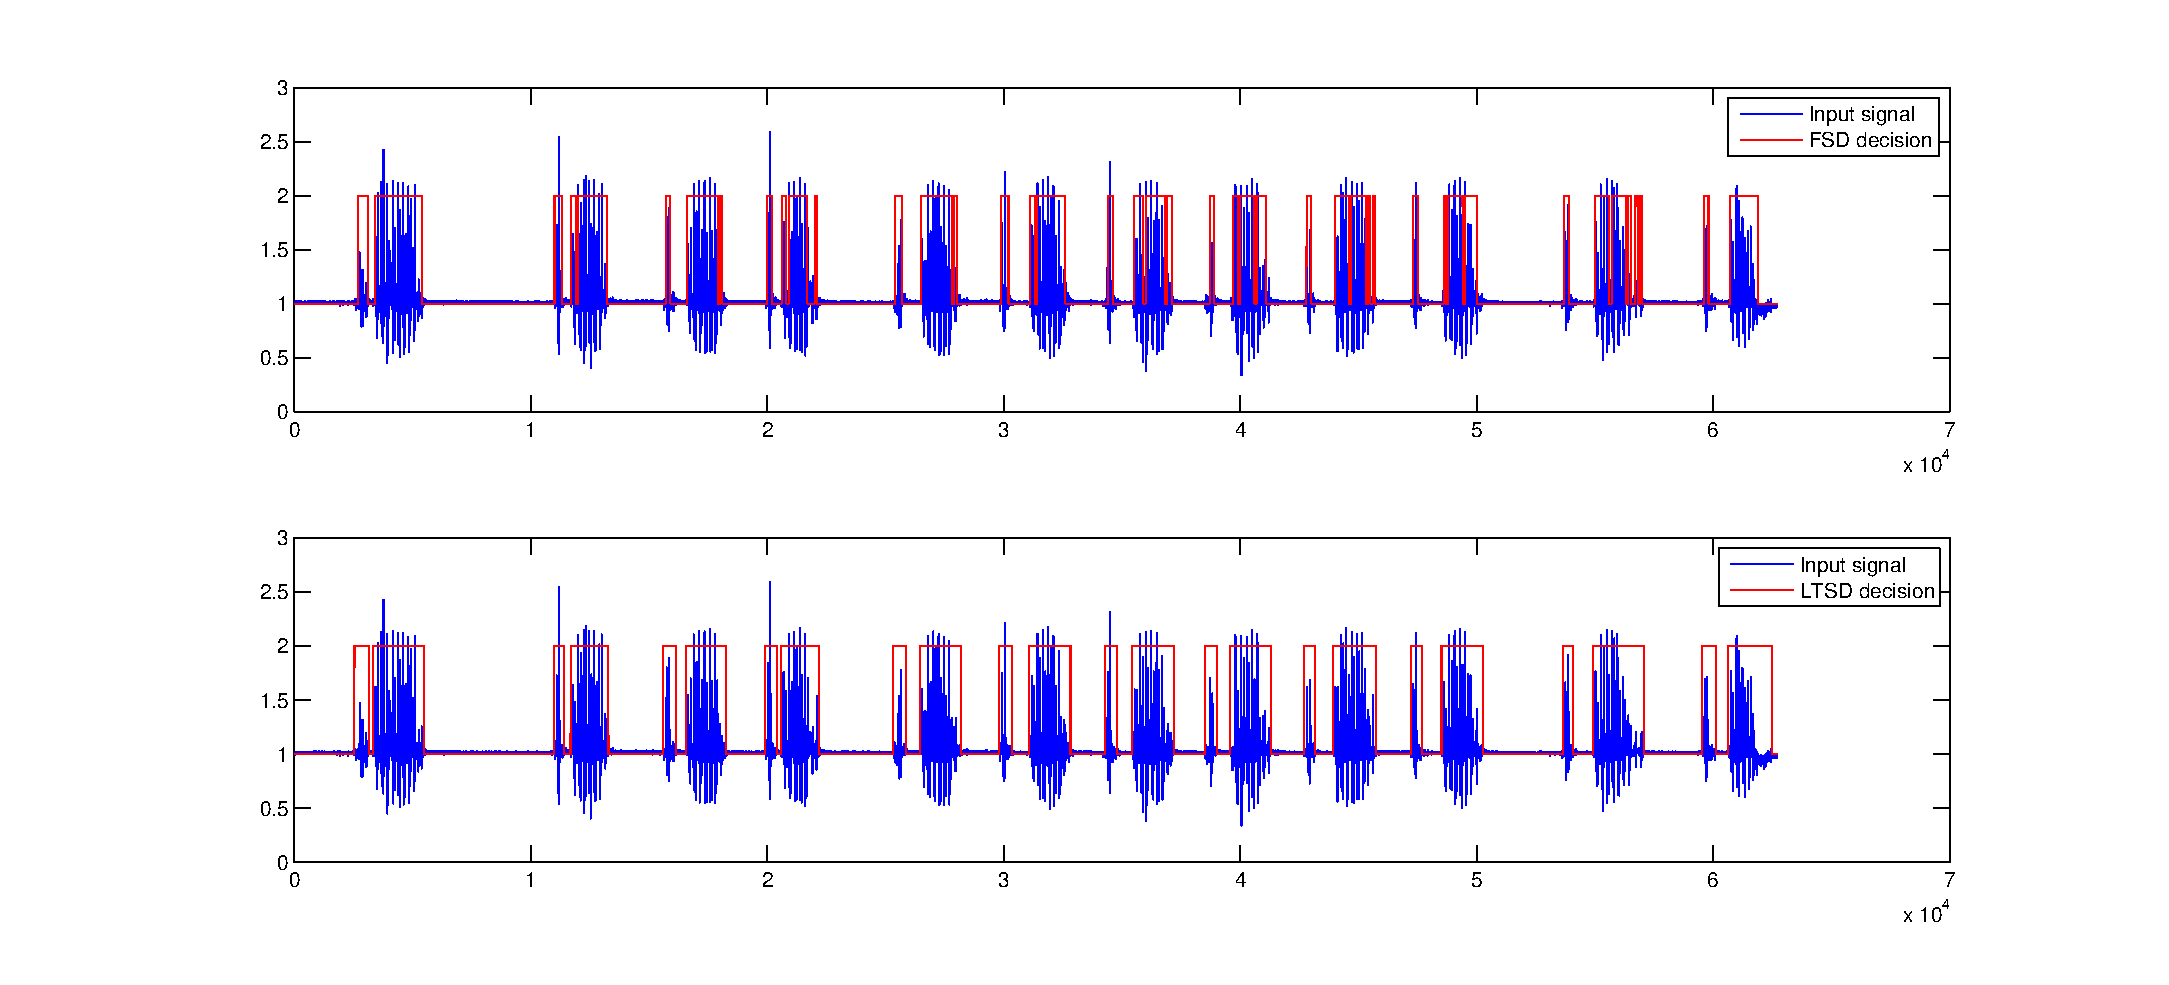
\epsfig{file=figures/Synchronisation/activityDetection, width=18cm}
	\caption{Activity Detection with FSD and LTSD Algorithm.}
	\label{fig:activityDetection}
\end{figure} 

The LTSD method has a better decision rate than FSD method because it is designed to work under condition where the SNR is low, i.e the signal present large noise\cite{A.Olivares2013}. In our case, we want detect the differents cycles that corresponding to each repeat so the different peaks of activity inside each period can be a problema to do the detection correctly because really it is interpreted like noise for the detector. Thus, the LTSD method is more interesting for this type of signal.

Once we select the best method for the detection we tested several input signal for the detector: shank acceleration signal, absolute value of the shank acceleration signal and module of the shank acceleration signal. Finally, the best result was obtained when we used module of the shank acceleration signal because when this input signal is used in the resulting output signal is easier to distinguish the different episodes.

Furthermore, the motion activity detection was carried out for the right leg as well as left one. It is not necessary in some cases when the patient does the movements or activities quickly since the detected activity interval  include both movements in the same episode. However, when patient waits some time to step again in the same repeat, it is possible that some step is not  include in the interval thus the result would be erroneous. Therefore, to realise a general algorithm useful in whatever case we differentiate between both feet.

Once the cycles have been separated, we are going to detect the key points in the signals to do the synchronisation. 

On the one hand, the time point when the patient does the step in the platform is exactly when the person touches it, that is, the time point that corresponding with the first sample in the force signal with a value other than zero.

On the other hand, in the acceleration signal case, this fact happens in the second positive peak\ref{fig:pointdetectionAcc}. The reason is that when patient does a step, the first movement is to rise the leg, so the acceleration vector points upwards thus the great positive peak will be when the leg is in the máximum distance from ground.Then, there is a change of direction and it appears a negative peak in this trace. The immediate movement is to lower the leg and touch the platform, so when the patient puts his leg in the force plate there is a positive peak due to the acceleration vector is pointing upward again.\ref{fig:sinchronisedSignals}.

Now, we have to consider others aspects like the limbs with which the person start to walk. To do all more comfortable for the patients, it was not specified with which leg they had to do the first step, so we have to determinate automatically this fact. To realise this we calculate all interesting peaks in the right shank acceleration as well as left shank acceleration. Then, we identify first peak in time \ref{fig:startLeftRight}.

\begin{figure}[H]
	\centering
	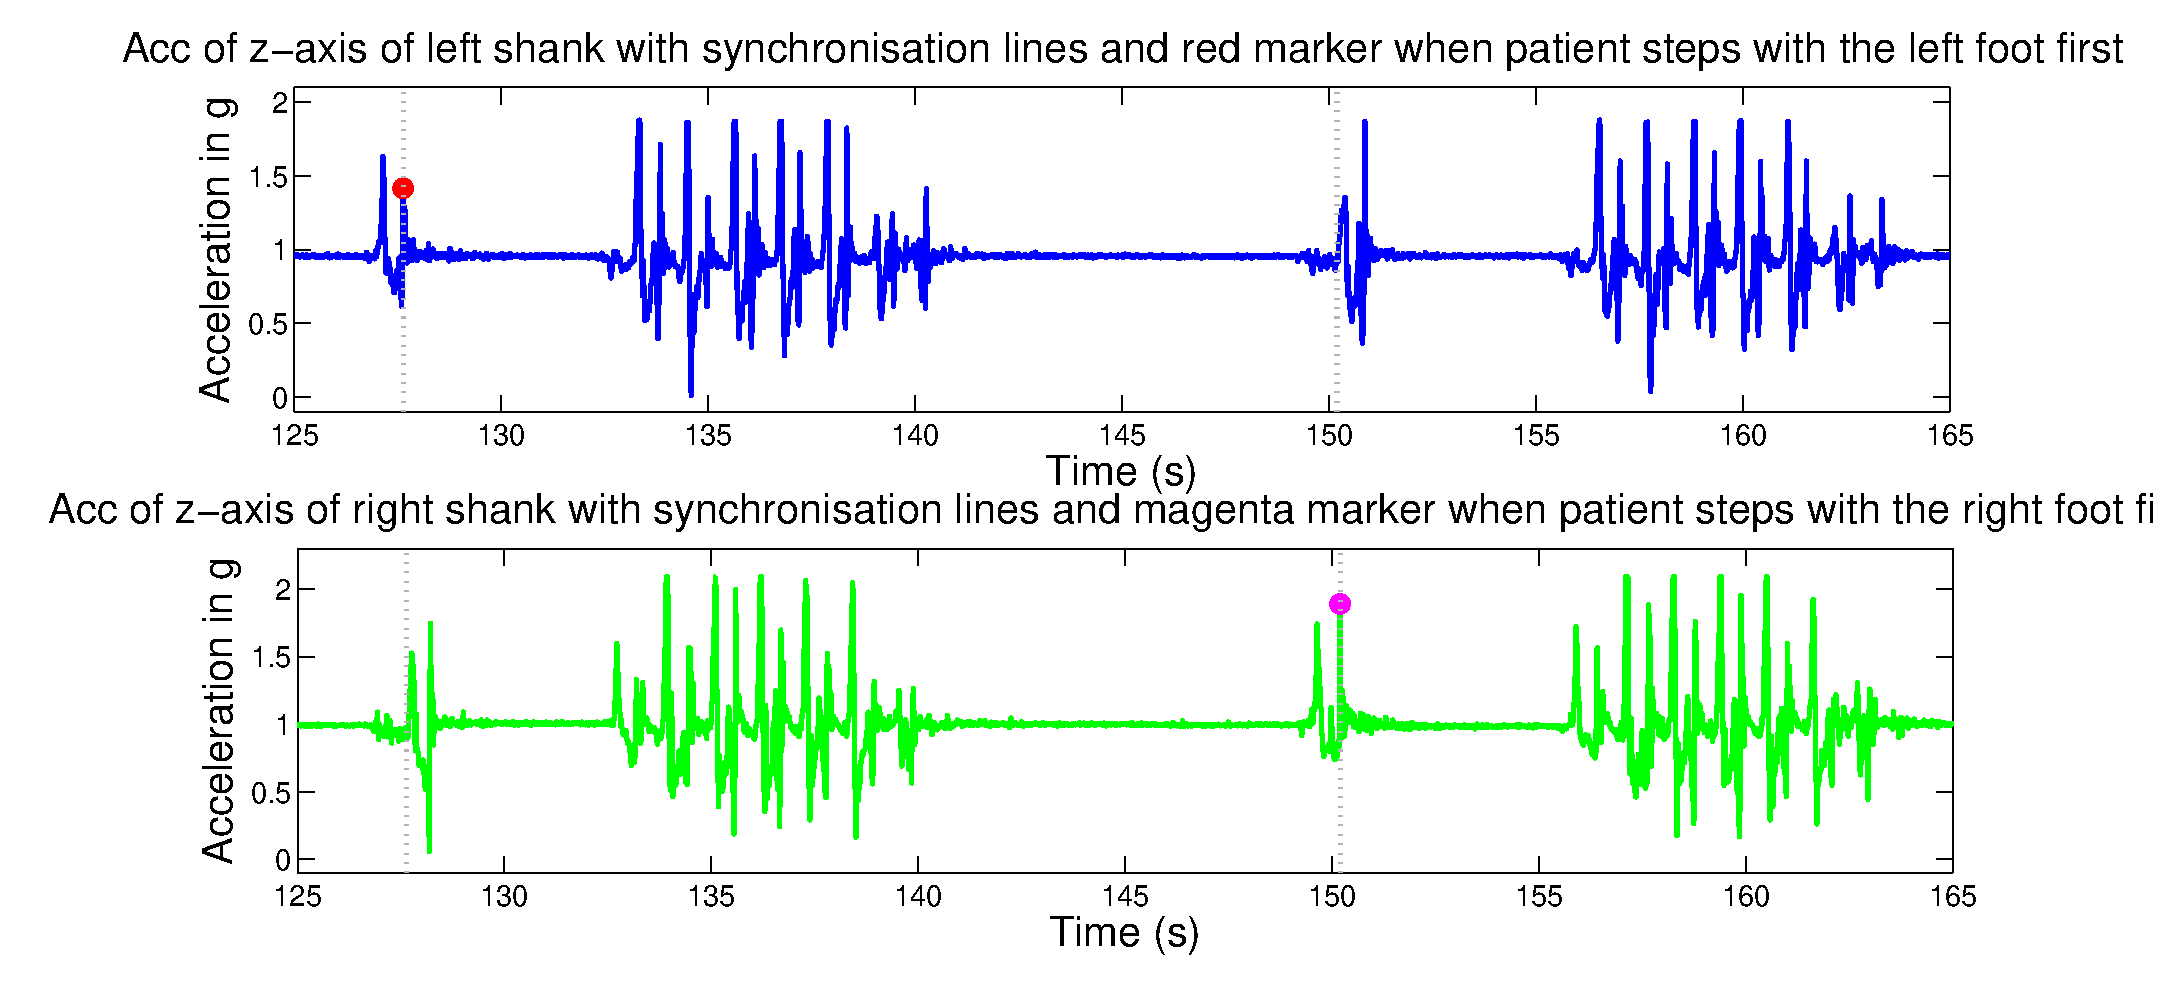
\epsfig{file=figures/Synchronisation/startLeftRight, width=18cm}
	\caption{Accelerometer signals when the patient starts to step with the left and right foot respectively.}
	\label{fig:startLeftRight}
\end{figure} 

Other important aspect is to consider the sample frequency. The sample frequency is 120 Hz in force plate signals and 200 Hz in GaitWatch signals. Thus, we have to reshape the Force Plate signals to match other signals.

All the key parameters and signals are saved using “time series”  for adding descriptive information to the fact.

Finally, we compare the peak detection for the synchronisation between the accelerometers signal and the gyroscopes signal. The behaviour of the gyroscope signal is clearer to the naked eye. We can sense there are a negative peak when the patient raises his leg to step. This is negative because the movement is upwards and the Z axes is pointing to the floor so the Angular Velocity is negative. The next positive peak of happends when the person touches the platform so this is the key point to use in the synchronisation\ref{fig:pointdetectionGyro}.

If we compare the behaviour of both signal, it makes sense because a peak of acceleration have to appear when there is a strong growth (or decrement) of the velocity, and this happends when the person go up or down the limbs\ref{fig:pointdetectionAcc}\ref{fig:pointdetectionGyro}.


\begin{figure}[H]
	\centering
	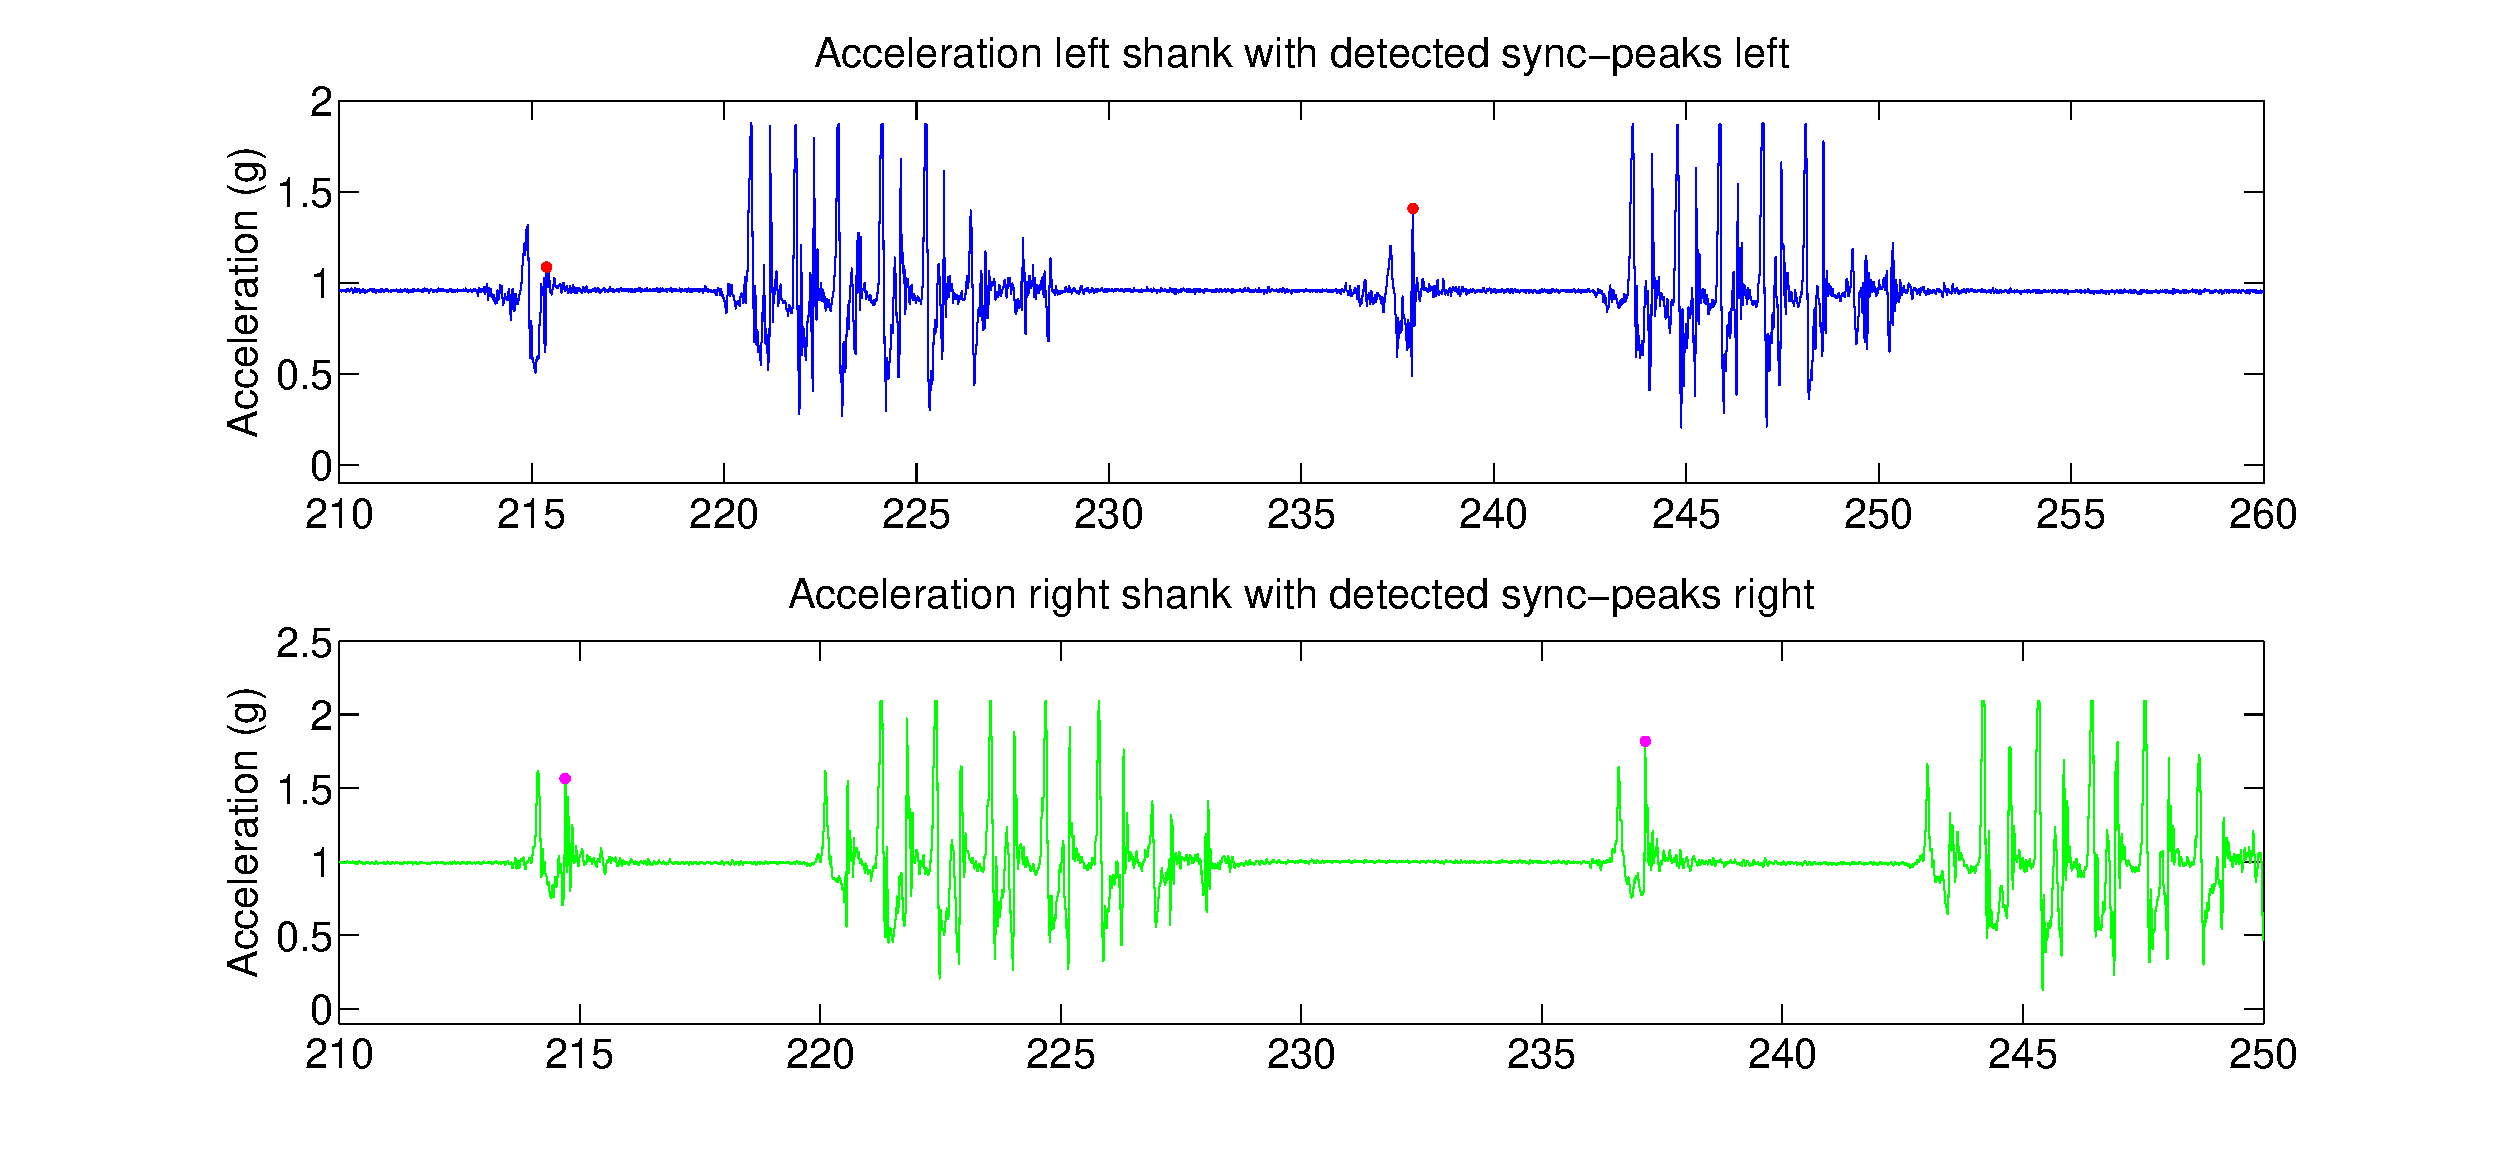
\epsfig{file=figures/Synchronisation/pointdetectionsynchronisation, width=18cm, height=10cm}
	\caption{Peaks detected for the Synchronisation in the Accelerometer signals.}
	\label{fig:pointdetectionAcc}
\end{figure}

\begin{figure}[H]
	\centering
	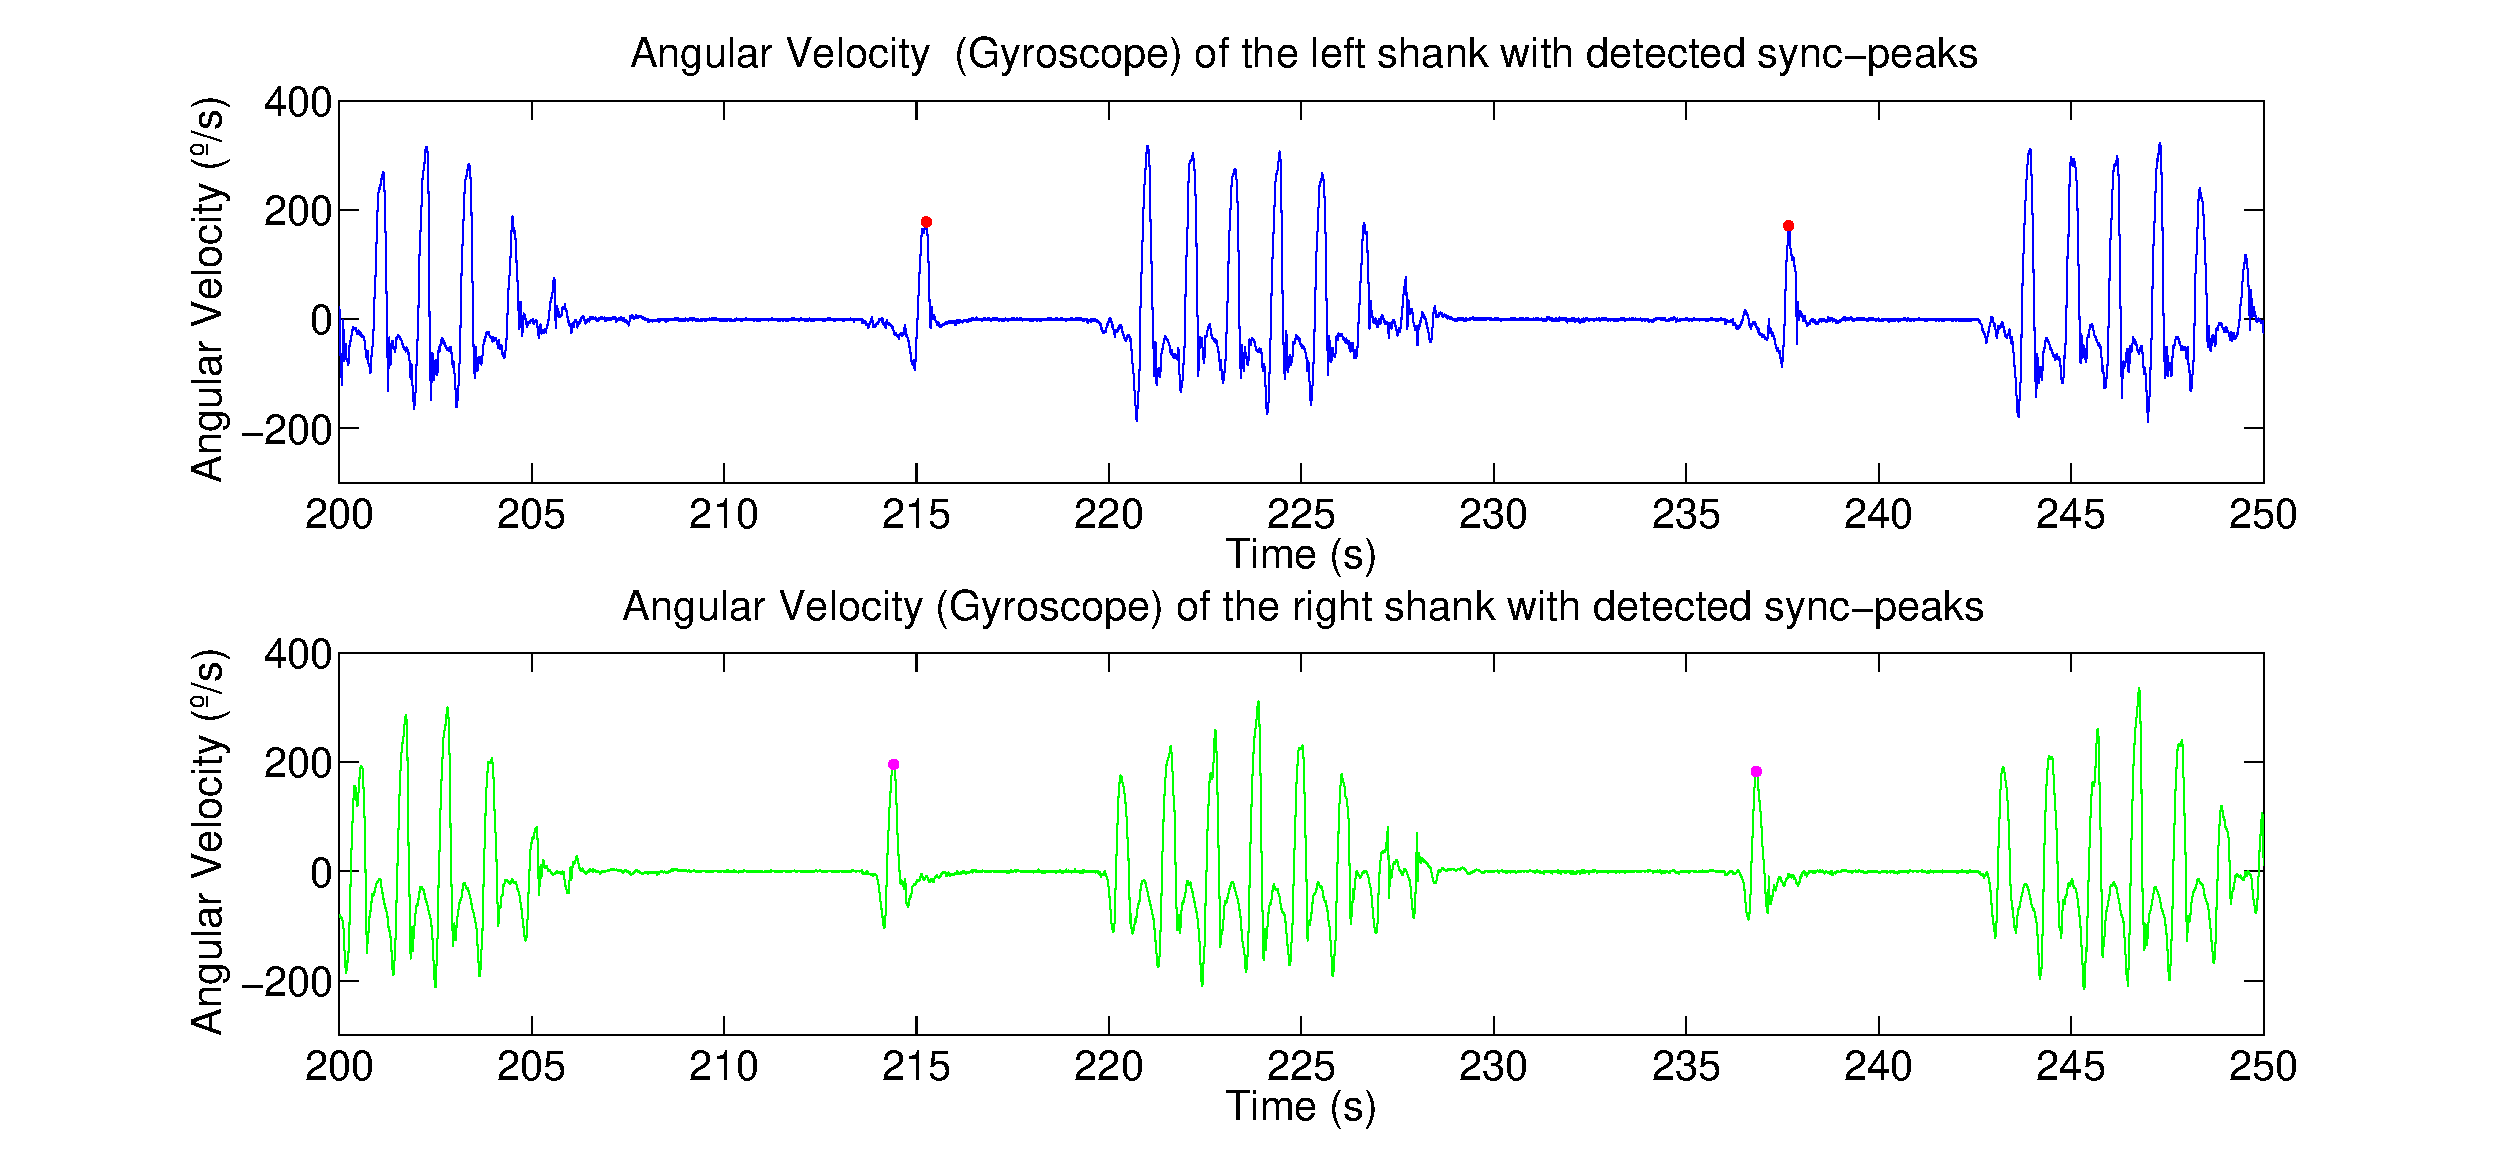
\epsfig{file=figures/Synchronisation/gyrosPointDetection, width=18cm,height=10cm}
	\caption{Peaks detected for the Synchronisation in the Gyroscope signals.}
	\label{fig:pointdetectionGyro}
\end{figure}

The correlation between the peaks detected with both systems is very high and the difference between the locations of the peaks are very small as well. This indicates that it was done correctly and these detected points are suitable to do the synchronisation. We can see this in the folllowing figures:

\begin{figure}[H]
	\centering
	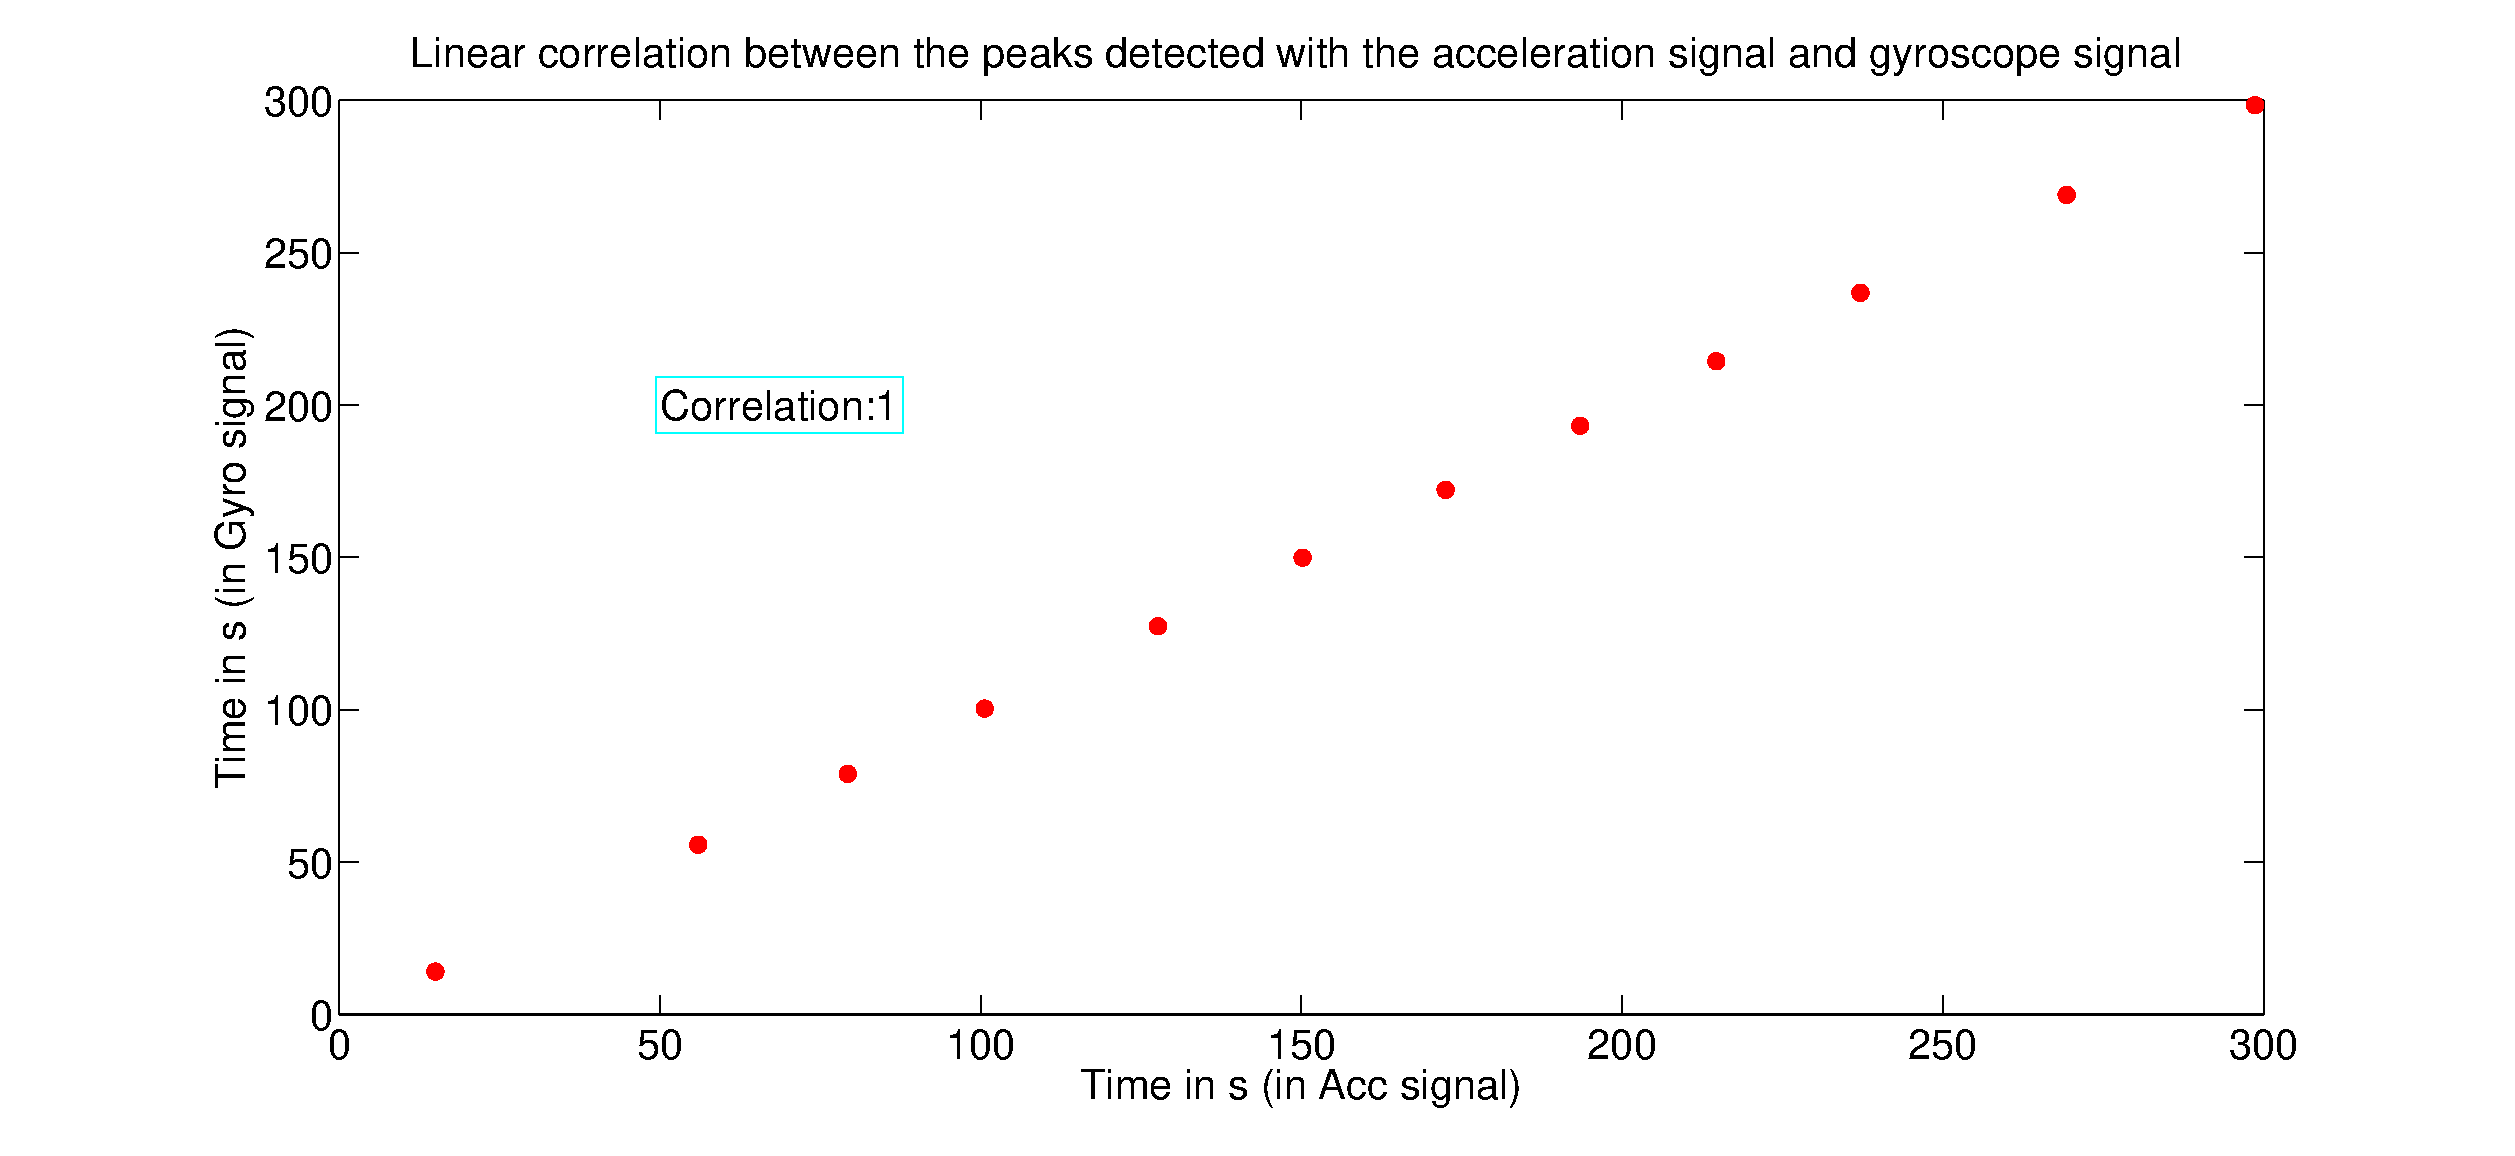
\epsfig{file=figures/Synchronisation/corrAccGyroPoints, width=18cm}
	\caption{Linear Correlation between peak Acc and peak Gyro used for the synchronisation.}
	\label{fig:corrAccGyroPoints}
\end{figure}

\begin{figure}[H]
	\centering
	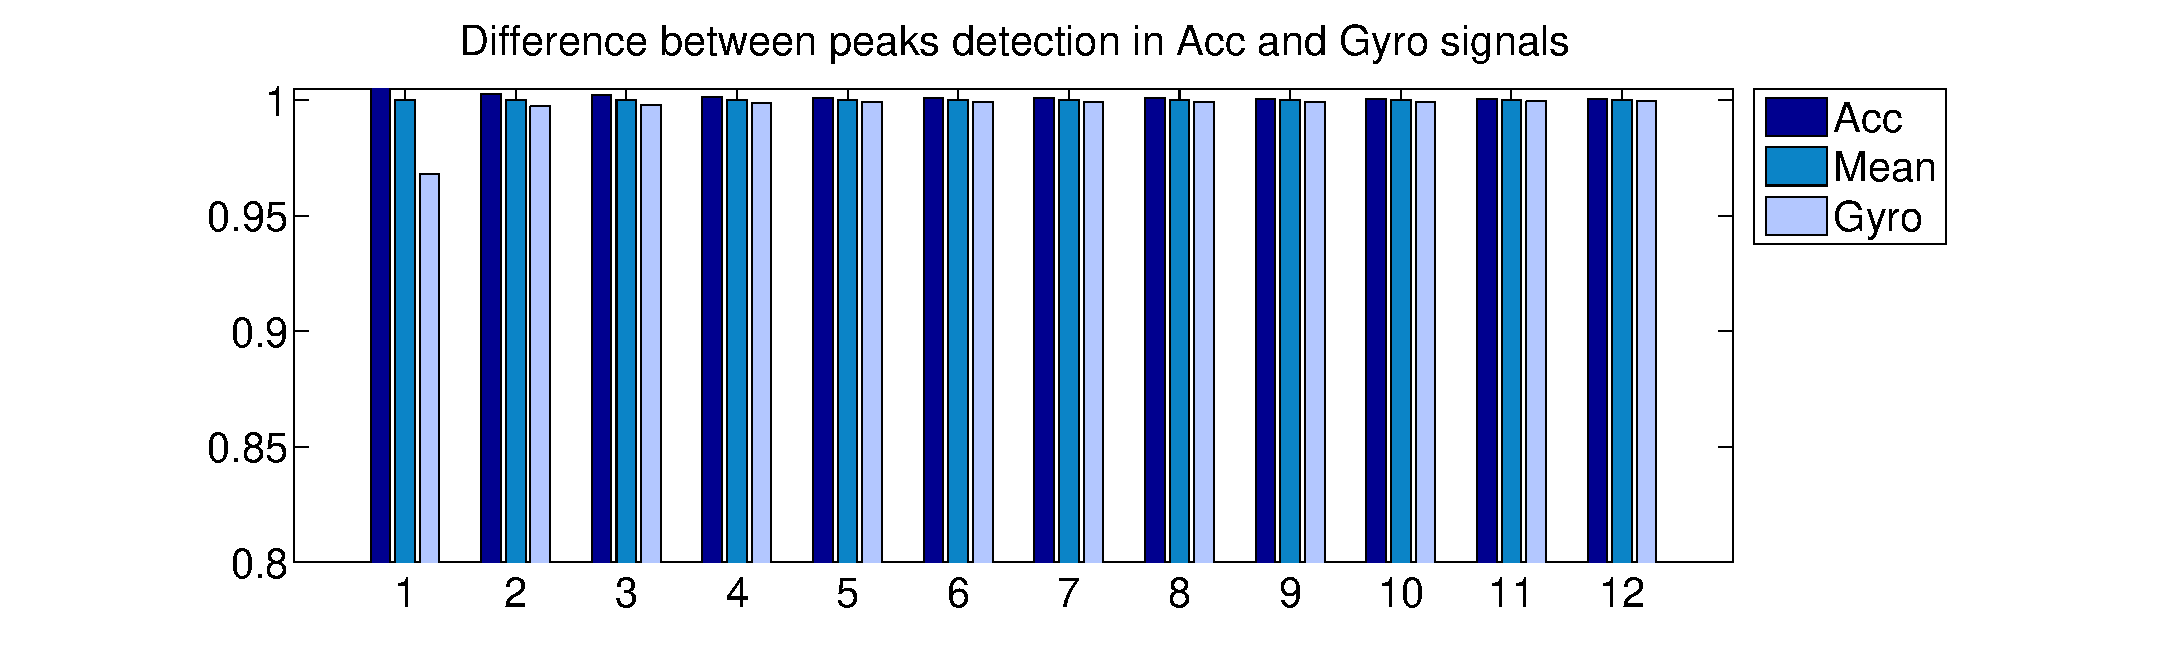
\epsfig{file=figures/Synchronisation/barDiagram, width=18cm}
	\caption{Comparation between points synchronisation detected with accelerometers and gyroscopes.}
	\label{fig:barDiagram}
\end{figure}


In \ref{tab:comparationAccGyro} table we can see that the mean of the difference between the peaks detected with the accelerometer and gyroscope signals is less than 0.5 second in all cases, so it is very small. Also, the correlation between them is very high and the probability of no correlation is smaller than 0.05 what want to say that the correlation is significantly different from zero.

\begin{table}[h]
	\caption{Comparation between the peaks detected with acceletometer and gyroscope}	
	\centering
	\begin{tabular}{|c|c|c|c|}\hline
		
		Patient 				& Average peaks difference 	& Corr 	& Prob 	\\ \hline
		ES39 & 0.3438			& 1.0									& 1.096 e-13					\\
		RK55	& 0.3014			& 1.0									& 2.720 e-13				\\
		RS46o & 0.2500			& 1.0									& 2.750  e-29					\\
		MM57	& 0.4970			& 1.0									& 3.480 e-26					\\
		WS42  & 0.3990			& 1.0									& 1.410 e-25					\\
		SW47	& 0.3615			& 1.0									& 2.190 e-25					\\
		TS40  & 0.2674			& 1.0									& 1.559 e-31				\\ \hline
	\end{tabular}
	\label{tab:comparationAccGyro}
	
\end{table}

Finally, the result of the synchronisation can be seen in following figure:

\begin{figure}[H]
	\centering
	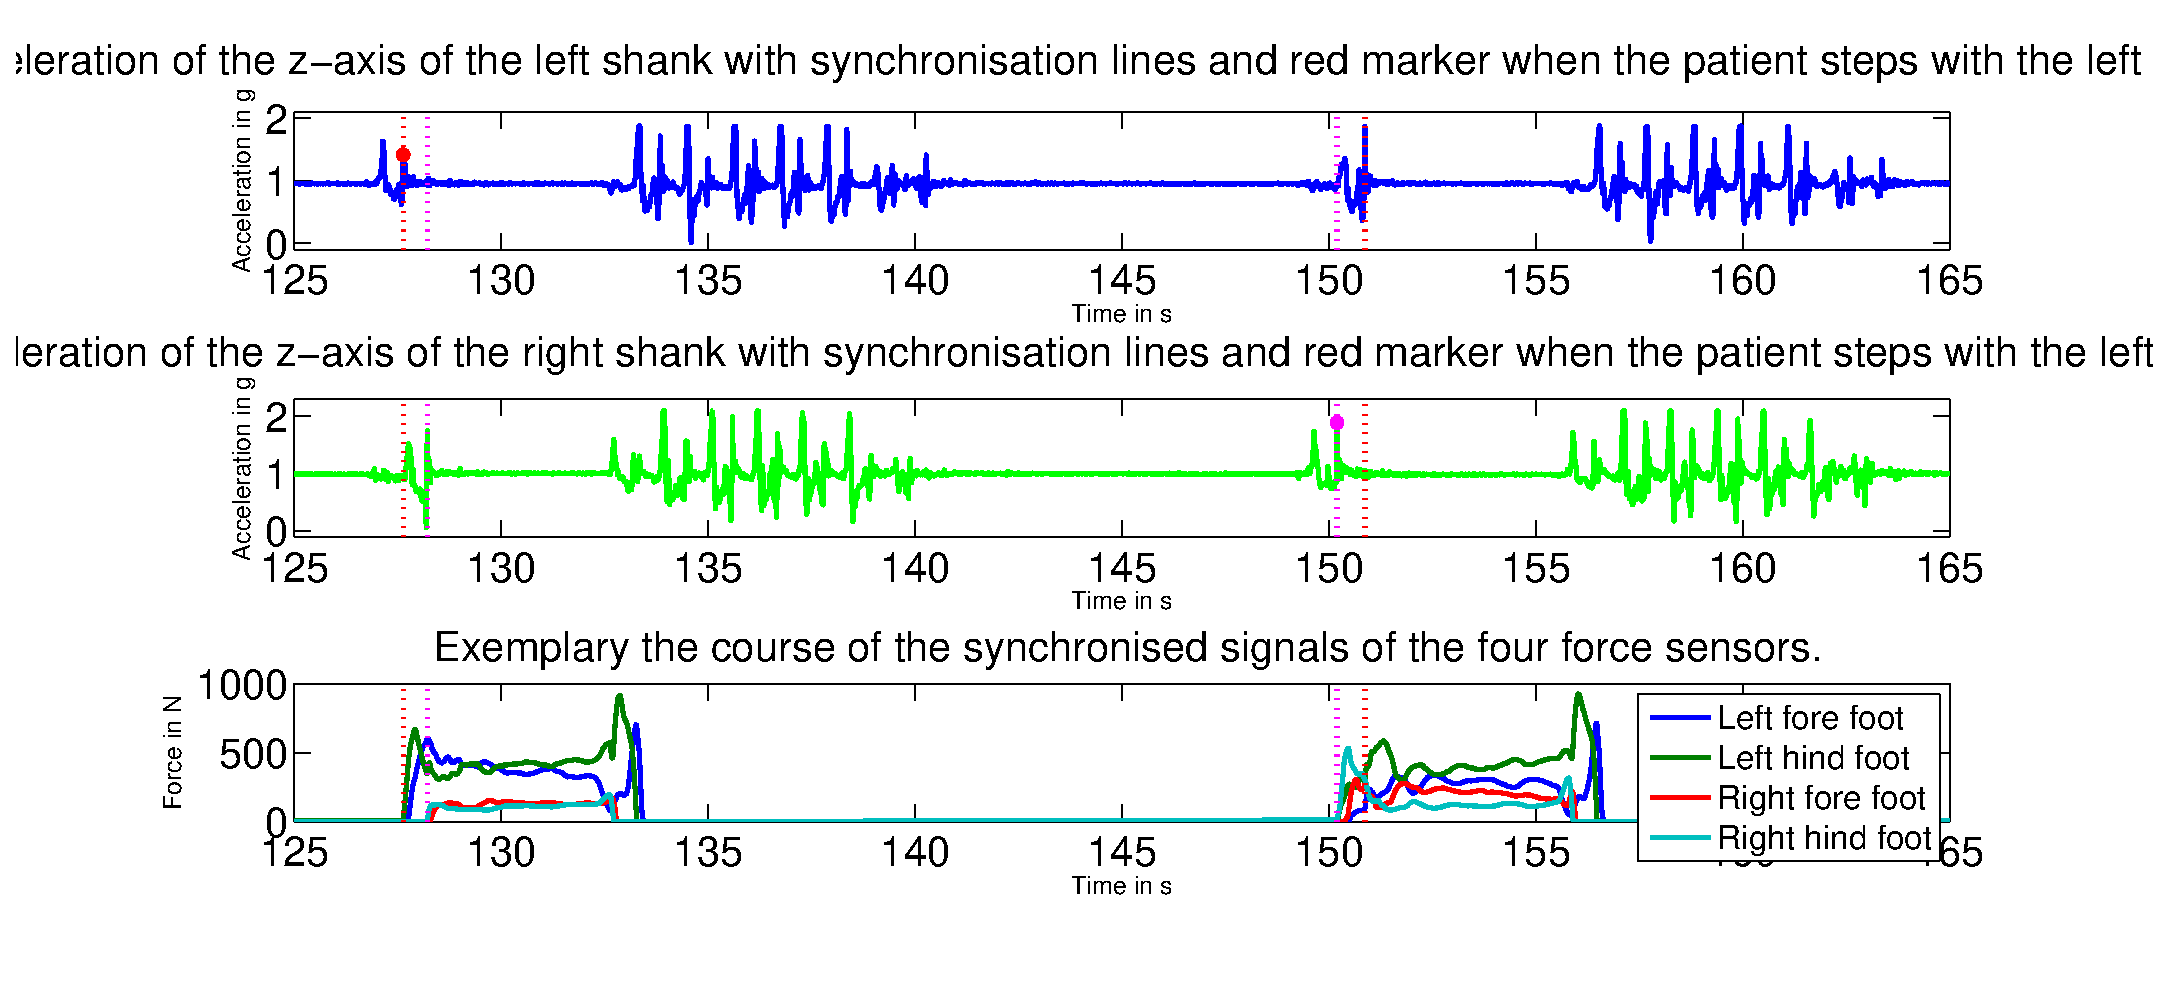
\epsfig{file=figures/Synchronisation/sinchronisedSignals, width=18cm, height=10cm}
	\caption{Synchronisation of the Force from the FP and Acceleration from the GW System .}
	\label{fig:sinchronisedSignals}
\end{figure}


\section{APA analysis}
\subsection{Introduction and chapter's structure}

Anticipatory postural adjustments (APAs)  represents balance control that help to stabilise and mobilise the body based on anticipation of forces accompanying voluntary movement such as volitional lifting of the foot during step initiation \cite{Mancini2010} . Step initiation requires a tight proprioceptive coordination between motor commands for postural adjustments and for stepping, so APAs act to accelerate the center of pressure over the stance foot immediately prior to gait \cite{Mancini2009} .

APAs, before gait initiation, are bradykinetic in advanced Parkinson’s disease and may be one of the factor associated with ‘start hesitation’ \cite{Mancini2009} .

Early identification in patients with PD is important because new neuroprotective medications are being tested to slow the progression of this disease and it is necessary to begin early in the disease, prior to significant loss of neurons \cite{Mancini2012} . 

Currently, the most common way to evaluate postural control in the clinic is to use clinical rating scales that are limited by clinician bias, insensitivity to mild impairments and poor reliability. These limitations are serious problems for clinicians and researchers who want to monitor the disease progression, determine intervention efficacy or treat people with mild balance deficits \cite{Mancini2012} .

Technology avaiable for clinicians and researchers to mesure APAs is generally force plate for the analysis of center of pressure. However, force plate is quite large and expensive and requires a proper installation that may not be practical for clinical use. Thus, Body-worn accelerometers have been proposed as a portable, low-cost alternative to a force plate for measurements of postural sway\cite{Mancini2012} .
 
Therefore, along this chapter we will do a comparative study of the measurements obtained of the force plate as well as accelerometers that make up the Gait Watch system. Also, we will compare these measurements with gyroscopes data that form part of this system too, in order to determine what sensors give us the more accurate results.

\subsection{FP and GW Signals}
As we said in the before chapter, leg's acceleration in the Gait Watch System as well as force in the Platform System are the most accurate signals to detect when the step happens. This is very important to do the synchronisation of the all signals of the system. However, the most interesting signals since a medical point of view are the trunk acceleration and the displacement of the center of pressure.

This is because we can observe the Anticipatory Postural Adjustments in these signals, i.e the body movements before stepping. According to prior studies and priori criteria it is thought that could be a good way to characterise the APAs.
Therefore, the first process to carry out is the analysis of the trunk acceleration and COP to determine if there is some pattern and whether we will be able to use them to obtain information about the patients.

The first step that needs to be carried out is establish the axes in the platform to define the position over it. The X axis points forward, not existing negatives values because the range is between 0 and 510 mm, that is the platform’s dimension in this direction. The Y axis is pointing to the right of the patient, so the positives values indicate a movement toward right with regard to the midline. Comparably, the negatives values are found when the movement is toward the left\ref{fig:axesFP}.

\begin{figure}[H]
	\centering
	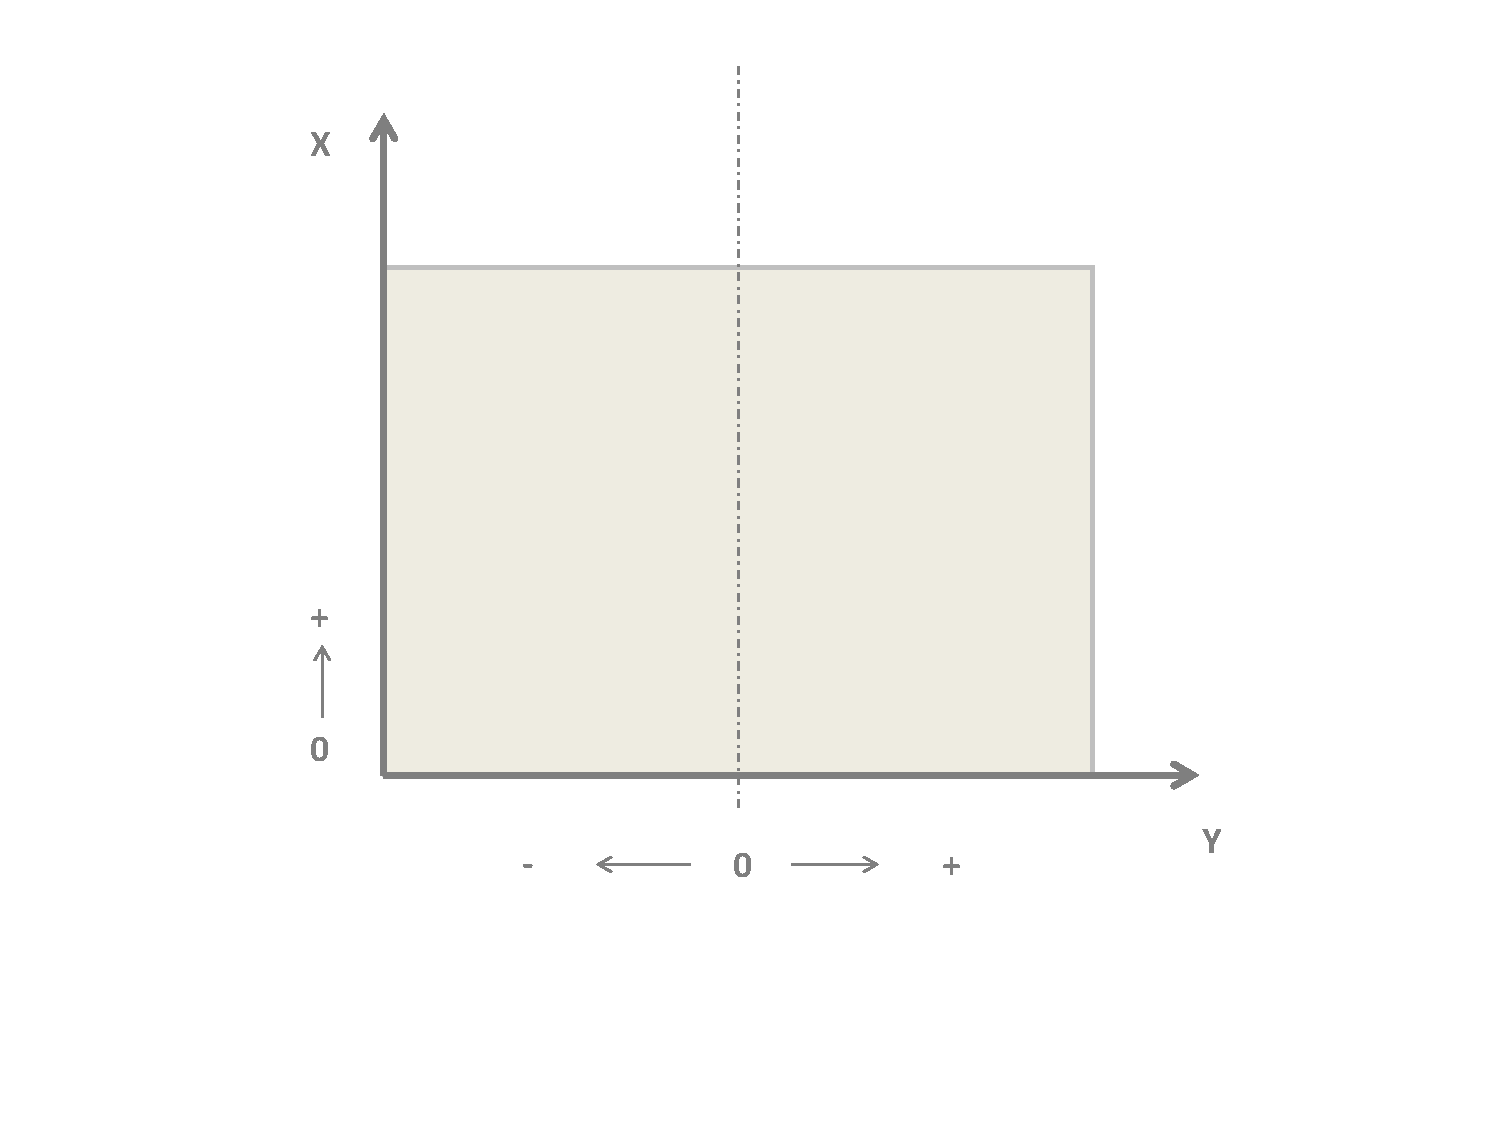
\epsfig{file=figures/APA_analysis/axesFP.pdf, width=18cm}
	\caption{Definition of the axes in the Platform.}
	\label{fig:axesFP}
\end{figure}

Now, for the GaitWatch System we have to determine the orientation of the axes of the body frame that we wish to use, as well as the orientation of the rotation around those axes. The most popular configurations is to set the X axis pointing forwards, the Y axis pointing to the right and the Z axis pointing down. This configuration follows the rule of the right hand for the orientation of the axes and the corkscrew rule for the rotation. \cite{OlivaresBotzel2013}

Since we will be using the GaitWatch device to monitor gait, then we need its X axis to point to the front of the patient, the Y axis pointing to the right  of the patient, and the Z axis to the floor\ref{fig:axesGW}.\cite{OlivaresBotzel2013}

\begin{figure}[H]
	\centering
	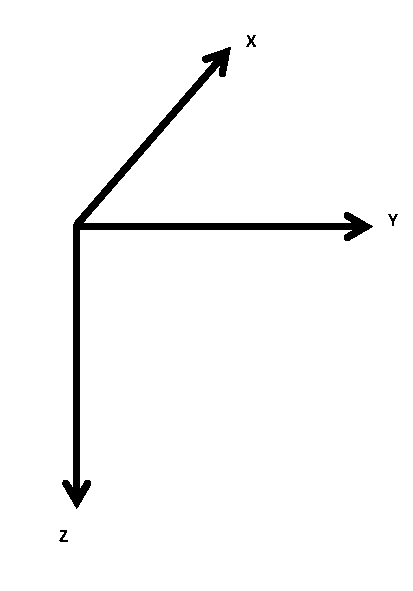
\epsfig{file=figures/APA_analysis/axesGW.pdf, width=18cm}
	\caption{Definition of the axes in the accelerometers ans gyroscopes.}
	\label{fig:axesGW}
\end{figure}

Once we have identified the axes of the accelerometers, we now proceed to identify the axes of the gyroscopes and their orientation. By convention, as it is depicted in figure 2.1, the sense of the rotation around a given axis is positive when the axis is pointing forwards (from the perspective of the user) and it is turned to the right. So, in this case the rotation is positive toward right\ref{fig:axesGWGyro}. Analogously, the rotation is negative when it is turned to the left  \cite{OlivaresBotzel2013}

\begin{figure}[H]
	\centering
	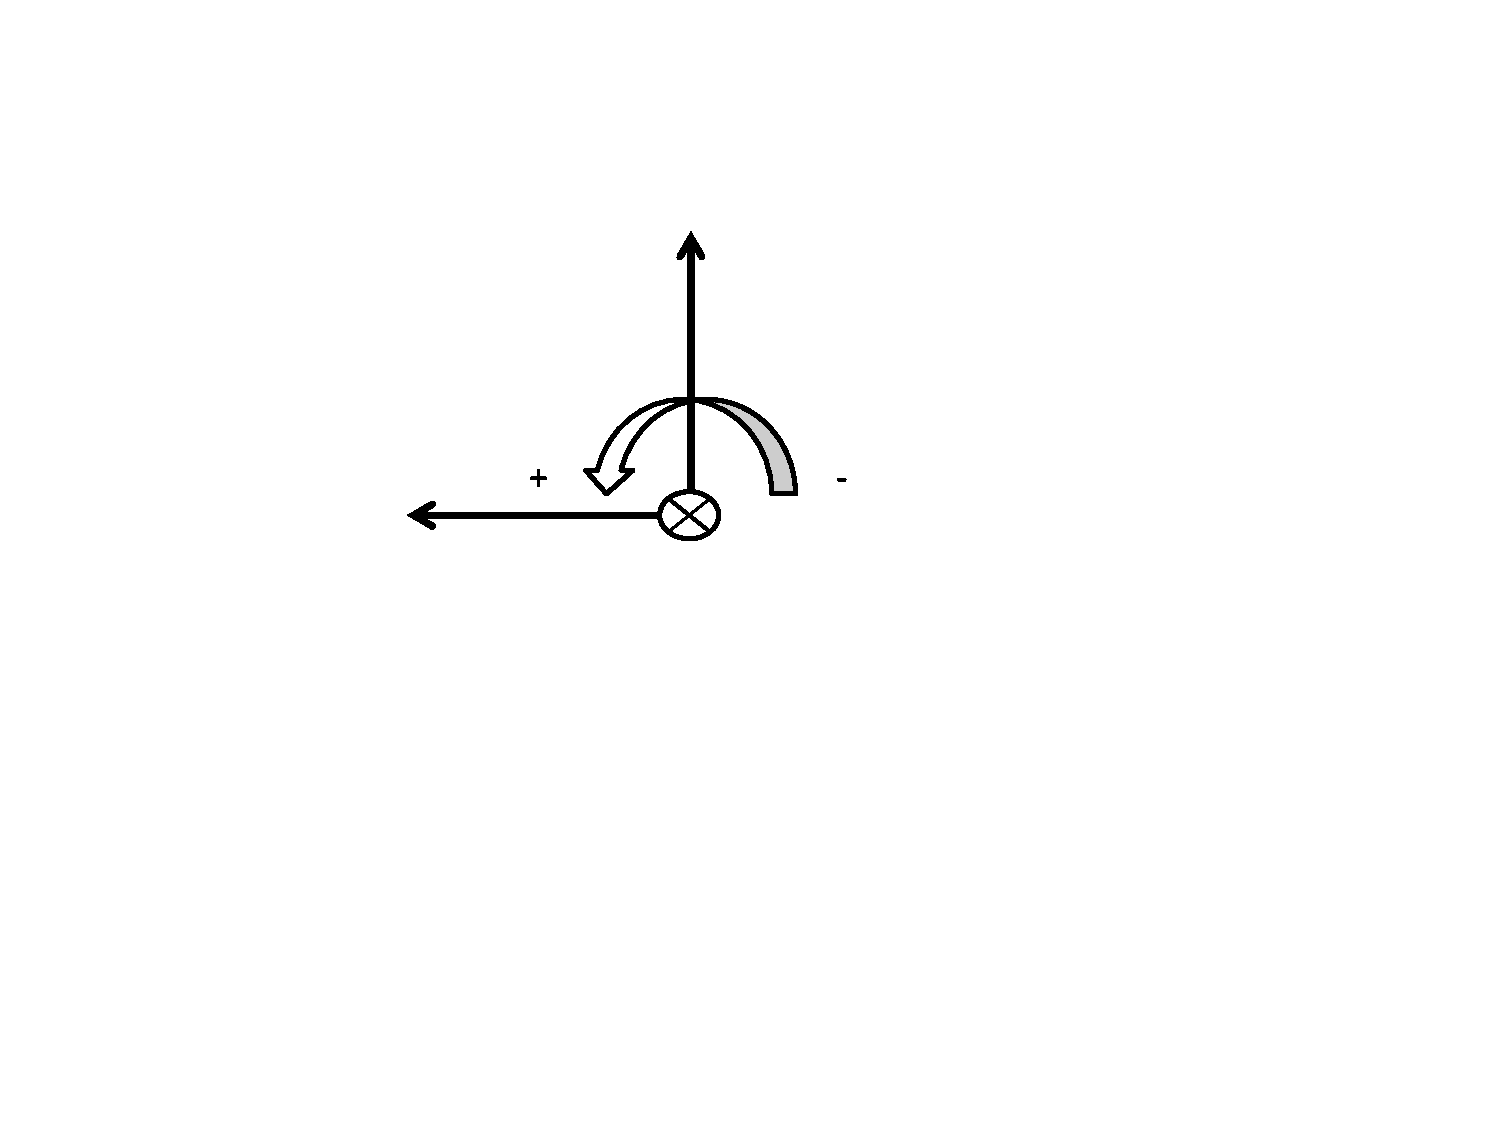
\epsfig{file=figures/APA_analysis/axesGWGyro.pdf, width=18cm}
	\caption{Orientation of the axis rotation in gyroscopes.}
	\label{fig:axesGWGyro}
\end{figure}


We have to differentiate between the front-back movement and the right-left movement. In the first of the case, we have the acceleration in X axis and the Antero-Posterior COP. In the another case, the movement is traced by the acceleration in Y axis and the Medio-Lateral  COP.

Whether we focus in the Antero-Posterior movement, the body is displaced forward while the step is being completed. Thus, the center of mass is shifted backward in this period of the movement. In the case of center of pressure, we can find first  movement backward to gain momentum and after that  COP moves forwards under the stance of the foot\ref{fig:AP_AccXtrunk}.

Since kinematic point of view, the trunk is moved anteriorly while the patient steps. Therefore, there will be a peak of acceleration in the X axis pointing forward, so we will find a ‘negative’ peak at this moment because the acceleration vector points in the opposite direction to the movement. After that, there is a positive peak that corresponding with the direction change just when the step finishes. 

Also, we can observe a pattern due to all movements before stepping follows a only trace approximately. So, if we observed the trunk signals when the patient starts with the right and left feet, we see the following signals:

The pattern of the acceleration in the X-axis (anterior-posterior movement) is always the same, regardless of the leg which the patient starts to walk. \ref{pattern_AP_acc}.

Moreover, we discern differences in the Medio-Lateral direction regarding the foot with which the step is done\ref{patter_ML_acc_right}\ref{patter_ML_acc_left}. 

If the patient starts to step with the right foot, the center of mass is accelerated toward left because the major body heigh is located in the foot over the ground. However, the center of pressure is shifted toward right and then the COP displaces mediolaterally to left, toward the foot is contact with the ground. For the acceleration in the Y axis, there is a negative peak because the movement is towards right and the acceleration vector points in the opposite direction, with negatives values. After this, we find a negative peak due to the change of direction. \ref{fig:ML_AccYtrunkNegative}

If the patient starts to step with the left foot, the movements are the same than in the prior case unless the movement directions are just the opposite. We can perceive this in \ref{fig:ML_AccYtrunkPositive}

To sum up, we have to differentiate between the foot which the step is done (stepping foot) and the foot over the ground (stance foot) to understand the behaviour of the APAs. The center of mass (COM) is shifted toward the stance foot to maintain the equilibrium during the balance phase. The center of pressure (COP) is divided in differents phases. Firstly, the COP moves toward the stepping foot and backward to generate the momentum to step (S1 period). Hereafter, the COP is displaced toward the stance foot. This happens at time when the other foot is in the air (S2 period). Finally, the COP moves forward and under the stance foot(S3 period). 
 
                 

GYROSCOPE

\subsection{PCA}
One of the most difficulties inherent in multivariate stadistics is the task of the features extraction to obtain the most relevant information from the original data and represent that information in a lower dimensionality space.

PCA is a qualitative rigorous method for achieving this and it has been widely applied in gait analysis both for the reduction of redundant information and the interpretation of multiple gait signals\cite{PCA}.

This method attempts to represent the data efficiently by descomposing a data space into a linear combination of a small collectionof bases collection of bases consisting of orthogonal axes that maximally decorrelate the data\cite{Jeon}.

Given  set of centered N-dimensional training gait samples 
$ x_{j}, j=1,...,M     x \in$ such that $ R_{N} $ and $ R=\sum_{k=1}^{M}x_{j}=0 $
	
Where M represents the number of gait samples and N is the number of input values. The $ x_{j} $ vectors are aligned in the data matrix X.
\begin{figure}[H]
	\centering
	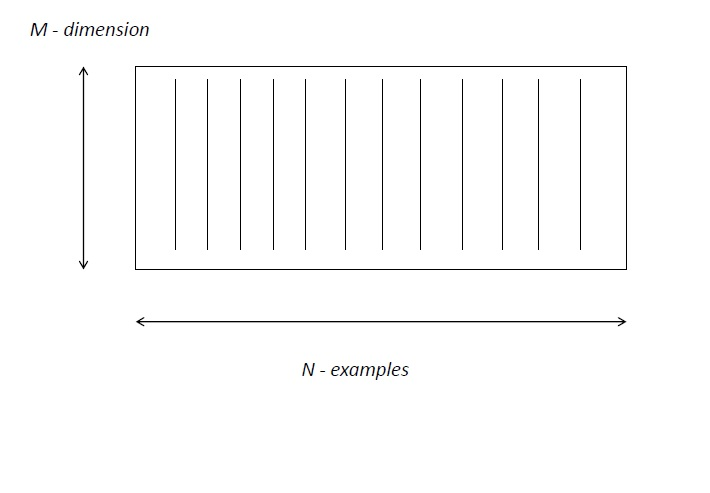
\epsfig{file=imagenes/PCA.jpg, width=18cm}
	\caption{Data matrix X with M rows and N colums.}
	\label{fig:matrixPCA}
\end{figure}

The projection of the j-th vector $ x_{j} $ onto the vector 'u' can be calculated in the folowing way:

\begin{equation}
	\label{projections}
	p_{j}=\overrightarrow{u}^{T}\overrightarrow{x}_{j}=\sum_{i=1}^{N}u_{i}x_{ij}	
\end{equation}

We want to find a direction 'u' that maximizes the variance of the projections of all input vectors. That funtion to maximize is:

\begin{equation}
	\label{maxfunction}
	J^{PCA}(\overrightarrow{u})=\sigma^{2}(p_{j})=\dfrac{1}{M}\sum_{j=1}^{N}(p_{j}-\bar{p})^{2}=...=\overrightarrow{u}^{T}C\overrightarrow{u}	
\end{equation}

Where C is the covariance matrix of the data matrix X.

$$C=\dfrac{1}{N}\hat{X}\hat{X}^{T}$$

Using the technique of Lagrange multipliers, the solution to the maximization problem is to compute the eigenvectors and eigenvlues of the covariance matrix.

Thus, we have to solve the following eigvector problem:
\begin{equation}
	\label{eigenproblem}
	\Lambda U=C^{'} U
\end{equation}

In such a way the orthonormal matrix U contains the eigenvectors $u_{1}, u_{2},...u_{N}$ in its colums and the diagonal matrix $\Lambda$ contains the eigenvalues $\lambda_{1}, \lambda_{2},...,\lambda_{N}$ on its diagonal.

The eigenvalues and the eigenvectors are arranged with respect to the descending order of the eigen values, thus $\lambda_{1}\eqslantgtr\lambda_{2}\eqslantgtr...\eqslantgtr\lambda_{N}$

Therefore, the most variability of the input random vector is contained in the first eigenvectors. Hence, the eigrnvectors are called principal vectors.

So U can be used as a linear transformation to project the original data of high dimension into a space of lower dimension.

$$P=U^T\bar{X}$$

In terms of gait feature extration by choosing the first fwo eigenvectors, PCA can directly perform the dimensional reduction\cite{Jeon}.

\subsection{Results discurssion}
		

	
	\clearemptydoublepage
	\bibliographystyle{unsrt}
	\bibliography{biblio}
	
	\clearemptydoublepage
\end{document}